\documentclass[]{book}
\usepackage[paperwidth=6in, paperheight=9in]{geometry}
\usepackage[overload]{textcase}
\addtolength{\oddsidemargin}{0.375in}
\addtolength{\evensidemargin}{-0.375in}

\newcommand{\blankpage}[1]{
    \newpage
    \thispagestyle{#1}
    \mbox{}
    %\newpage
}
\usepackage{graphicx}

\usepackage{floatpag}
\floatpagestyle{empty}
\rotfloatpagestyle{empty}

\renewcommand{\chaptermark}[1]{\markboth{\slshape{#1}}{}}

\usepackage[nouppercase]{scrpage2}
\pagestyle{scrheadings}
\chead{\headmark}
\ihead[]{}

\usepackage{verse}

\newcommand{\makeTitlePages}[6]{
    \pagenumbering{gobble}
    \blankpage{empty}
    \blankpage{empty}
    \newpage
    \vspace*{\fill}
    {\centering\Huge\bf\centering #1
    \vspace*{\fill}

    \title{#1}
    \author{#3}
    \maketitle}

    \cleardoublepage
    \pagenumbering{roman}
    \setcounter{page}{7}
}

%% Patch for blank pages between chapters
%% which disables the current page style
\makeatletter
\def\cleardoublepage{\clearpage\if@twoside \ifodd\c@page\else
  \hbox{}\thispagestyle{empty}\newpage\if@twocolumn\hbox{}\newpage\fi\fi\fi}
\makeatother

\usepackage{multicol}
\usepackage{xcolor}
\usepackage{allrunes}
\usepackage{xstring}

\usepackage[nf]{coelacanth}
\usepackage[T1]{fontenc}
%% The font package uses mweights.sty which has som issues with the
%% \normalfont command. The following two lines fixes this issue.
\let\oldnormalfont\normalfont
\def\normalfont{\oldnormalfont\mdseries}

\noexpandarg\exploregroups
\newcommand\dwarvenSpace[1]{\StrSubstitute{#1}{ }{\textarm{.}}}
\newcommand\dwarvenFullStop[1]{\StrSubstitute{#1}{.}{\textarm{\tripleeye}}}
\newcommand\dwarvenA[1]{\StrSubstitute{#1}{a}{\textara{\oe}}}
\newcommand\dwarvenAA[1]{\StrSubstitute{#1}{\=a}{\textara{\oe}}}
\newcommand\dwarvenB[1]{\StrSubstitute{#1}{b}{\textarm{b}}}
\newcommand\dwarvenD[1]{\StrSubstitute{#1}{d}{\textarm{\o}}}
\newcommand\dwarvenG[1]{\StrSubstitute{#1}{g}{\textarc{\RR}}}
\newcommand\dwarvenH[1]{\StrSubstitute{#1}{h}{\textara{h}}}
\newcommand\dwarvenI[1]{\StrSubstitute{#1}{i}{\textara{\j}}}
\newcommand\dwarvenII[1]{\StrSubstitute{#1}{\=\i}{\textara{\j}}}
\newcommand\dwarvenK[1]{\StrSubstitute{#1}{k}{\textarc{g}}}
\newcommand\dwarvenL[1]{\StrSubstitute{#1}{l}{\textarm{y}}}
\newcommand\dwarvenM[1]{\StrSubstitute{#1}{m}{\textara{m}}}
\newcommand\dwarvenN[1]{\StrSubstitute{#1}{n}{\textara{d}}}
\newcommand\dwarvenO[1]{\StrSubstitute{#1}{o}{\textarc{\ng}}}
\newcommand\dwarvenTH[1]{\StrSubstitute{#1}{th}{\textarm{\th}}}
\newcommand\dwarvenR[1]{\StrSubstitute{#1}{r}{\textarm{m}}}
\newcommand\dwarvenS[1]{\StrSubstitute{#1}{s}{\textarm{s}}}
\newcommand\dwarvenT[1]{\StrSubstitute{#1}{t}{\textarm{\ae}}}
\newcommand\dwarvenU[1]{\StrSubstitute{#1}{u}{\textara{\ng}}}
\newcommand\dwarvenUU[1]{\StrSubstitute{#1}{\=u}{\textara{\ng}}}
\newcommand\dwarvenV[1]{\StrSubstitute{#1}{v}{\textarm{\r}}}
\newcommand\dwarvenZ[1]{\StrSubstitute{#1}{z}{\textarm{x}}}
\newcommand\dwarven[1]{%
	\large{%
	\lowercase{%
	\dwarvenFullStop{%
	\dwarvenSpace{%
	\dwarvenTH{%
	\dwarvenAA{\dwarvenA{%
	\dwarvenB{%
	\dwarvenD{%
	\dwarvenG{%
	\dwarvenH{%
	\dwarvenII{\dwarvenI{%
	\dwarvenK{%
	\dwarvenL{%
	\dwarvenM{%
	\dwarvenN{%
	\dwarvenO{%
	\dwarvenR{%
	\dwarvenS{%
	\dwarvenT{%
	\dwarvenUU{\dwarvenU{%
	\dwarvenV{%
	\dwarvenZ{%
		#1%
	}}}}}}}}}}}}}}}}}}}}}}}}}
	\normalsize
}

\newcommand{\dwarvenDef}[3]{%
	\item[#1] \emph{\color{gray}#2.} #3
%
	%\dwarven{#1}
}
\newcommand{\dwarvenDefOld}[3]{%
% 1 word
% 2 word type
% 3 definition
	%\item[#1] \dwarven{#1}
	\item[#1] \dwarven{#1}

\emph{\color{gray}#2}. #3
}

\newcommand{\dwarvenInscription}[1]{

\vspace{1em}
	\noindent
	\begin{center}
	{
		%\large
		\dwarven{#1}
	}
	\end{center}
\vspace{1em}

}

\newcommand{\divider}{
\vspace{1em}

\hfill
%\rule{3in}{0.5pt}
***
\hfill{}

\vspace{1em}
}

\makeatletter
\def\cleardoublepage{\clearpage\if@twoside \ifodd\c@page\else
  \hbox{}\thispagestyle{empty}\newpage\if@twocolumn\hbox{}\newpage\fi\fi\fi}
\makeatother

\usepackage{floatpag}
\floatpagestyle{empty}
\rotfloatpagestyle{empty}

\renewcommand{\chaptermark}[1]{\markboth{\slshape{#1}}{}}

\usepackage[nouppercase]{scrpage2}
\pagestyle{scrheadings}
\chead{\headmark}
\ihead[]{}

\usepackage{tocloft} % the tocloft package lets you redefine the Table of Contents (ToC)
\renewcommand\cftchappresnum{Chapter } % prefix "Chapter " to chapter number in ToC
\renewcommand\cftchapdotsep{\cftdotsep}
\renewcommand\cftchapnumwidth{5em}


\newcommand{\poem}[1]{%
	\addcontentsline{lot}{table}{#1}
}
\renewcommand{\listtablename}{List of Songs and Poems}


\begin{document}
\frontmatter
%\makeTitlePages{The Dwarf and the Sword of Purity}{}{Timothy Gurto}{2021}{}{}

%\newpage
%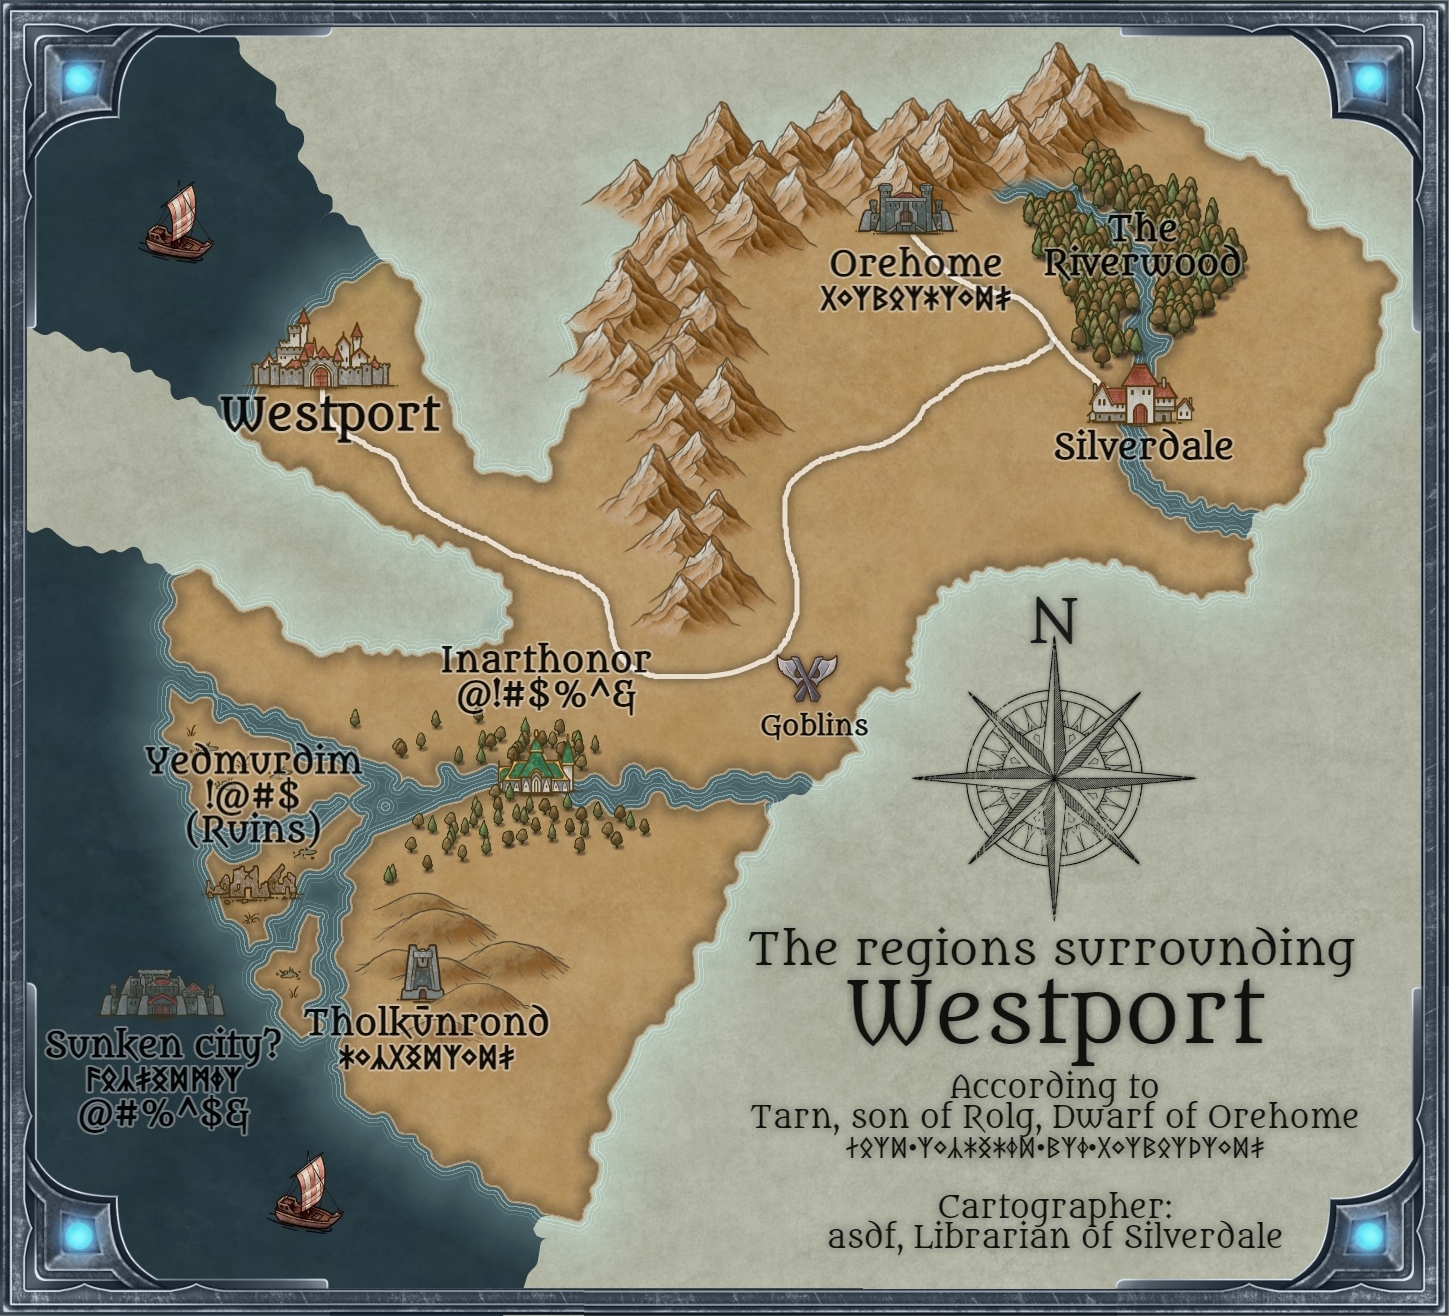
\includegraphics[trim=0 0 19cm 0, clip, width=\textwidth]{map}
%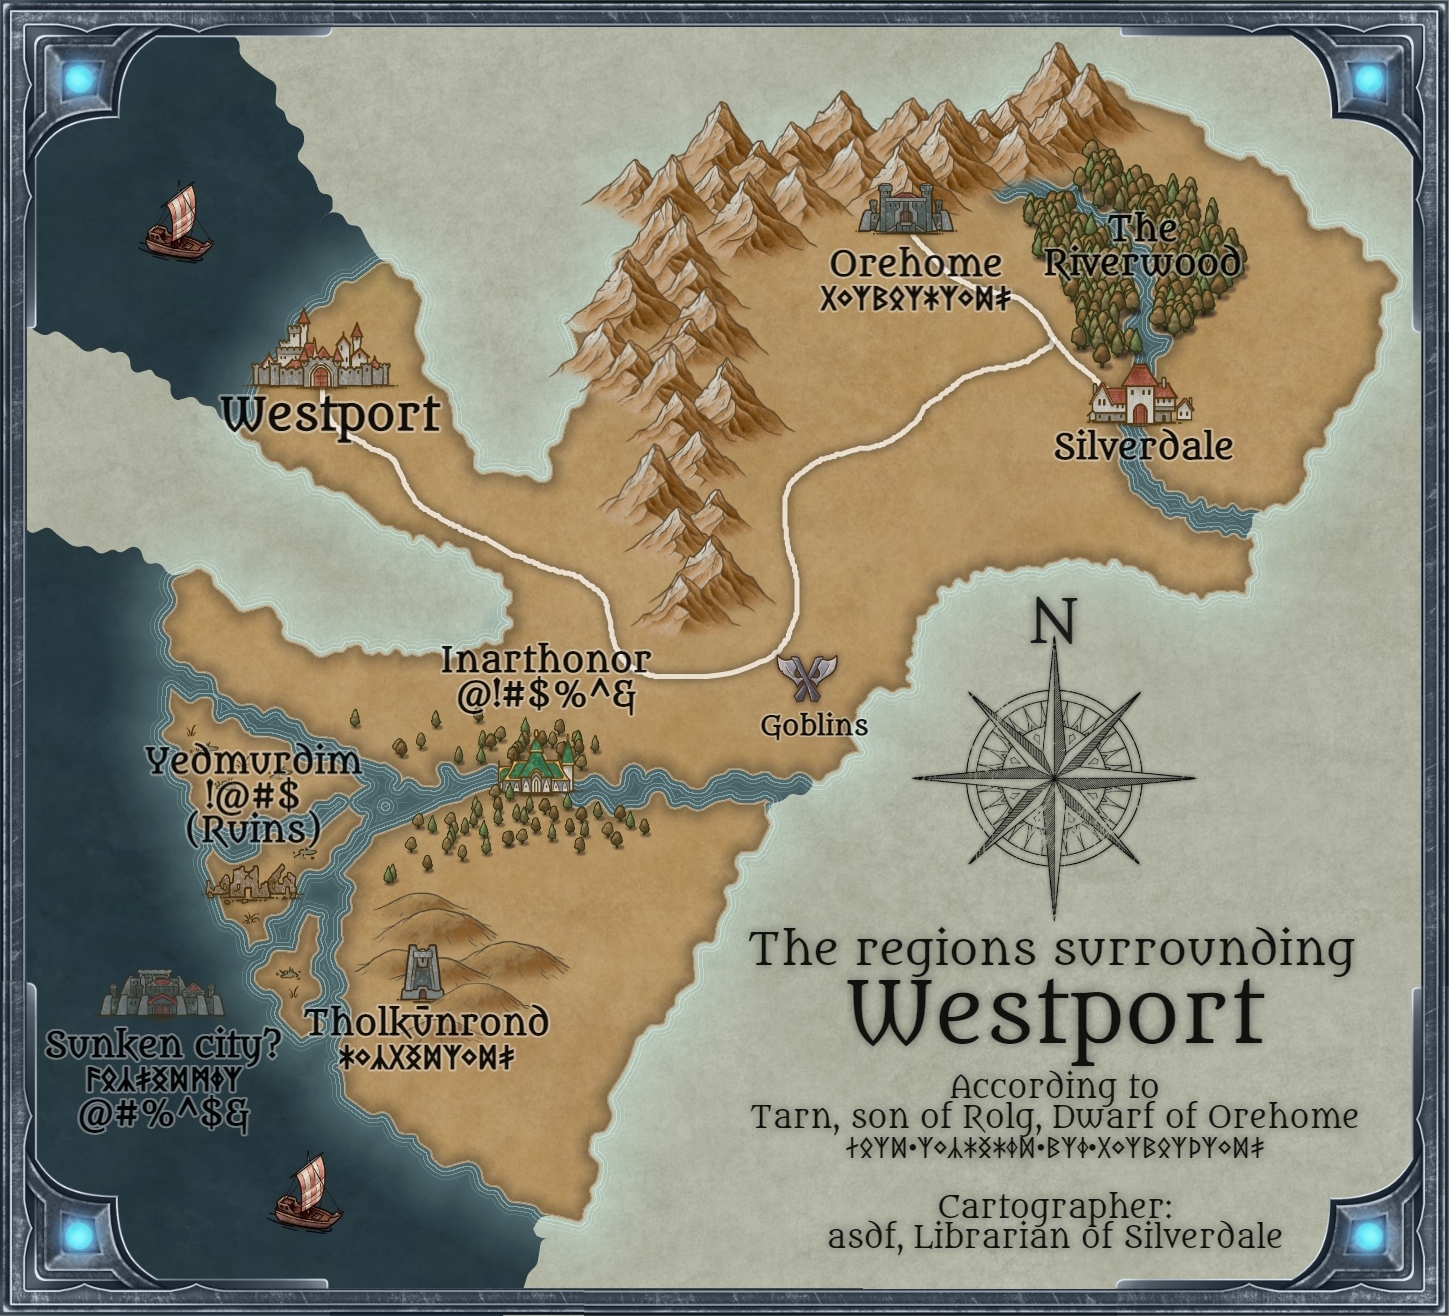
\includegraphics[trim=19cm 0 0 0, clip, width=\textwidth]{map}

\cleardoublepage
%\tableofcontents % commented out because the dots dirty the word count

%\addcontentsline{toc}{chapter}{List of Songs and Poems}
%\listoftables

\mainmatter
\chapter{Ripples in the Stone}
Tarn, son of Rolg, stood straight and still, his eyes peering over the city's entrance hall one last time before he ended his shift.  Guarding the city was as uneventful today as it usually was; the worst invaders Tarn had ever needed to repel from the city were bears and other wild animals.  In a more turbulent time he may have stood against an attacking horde, or have been part of an army marching off to fight for some great cause, but in this age of peace he stood \emph{inside} the gates, looking inwards.  Not that he minded---he was a dwarf, after all, and like most of his kind he was most comfortable nestled within the carved bosom of his mountain.

The entrance hall was cavernous and showy.  Wide columns stretched to the ceiling, so high that it was hard to see their tops among the distant dark.  The floor of the hall was tiled with polished marble, tapping sharply with each footstep from the dwarves going about their business.  Because it was so close to the main gate, over the generations this hall had developed into a marketplace for dealing with visitors from outside.  The city received only one or two traders per day, and so most of the merchants here still served the local dwarves.  Occupying the stall nearest to Tarn was a silversmith, whose tables were decorated with scales and stacks of coins and ingots.  Silver was the city's main export, and it was mined and smelted here in the mountain.  In the stall next to that one was a wood carver, selling ornaments.  There were larger markets deeper within the city, but this was the place to find those goods made to appeal to outside buyers.

The stone walls were engraved with elaborate patterns and images.  These walls were carved in-situ, straight into the original rock, and not placed there.  Marbled throughout them were veins of a pale blue mineral which the dwarves named simply Omunkorb, or ``Blue-ore'' in the language of Men.  Where the blue touched the engravings, it was polished to be bright and clear, so as to be more easily seen.  Omunkorb permeated much of the city, and the dwarves generally kept it intact wherever found: they could find no functional use for it, only decorative, and it had become a source of pride for them.  Thus was the city itself called \korbarthrond---``Orehome''.

A large inscription was engraved prominently on one of the high walls flanking the entrance hall, a message to citizens and visitors alike.  Its glyphs consisted of the hard, straight marks of the Dwarven script, adapted to be carved into hard materials.  The inscription read:
\dwarvenInscription{%
bamk azthu thaku trobu gi brolzolg\\%
dult korb krithsulb gorg izun gi kugzolg.}
Roughly translated, it means:
\settowidth{\versewidth}{Like ore, innate and polished in our walls,}
\begin{verse}[\versewidth]\poem{The exhortation of \korbarthrond}
Like ore, innate and polished in our walls,\\
should you be true yet shine within these halls.
\end{verse}

Tarn always enjoyed patrolling here, because it gave him an opportunity to admire the craftsmanship of those wall engravings.  The images depicted various stories from the history and myth of the city and her people, and they exhibited the care and love of fine work that most dwarves applied to their various vocations.  Guardwork afforded little opportunity for Tarn himself to scratch this itch, and so he instead found opportunities to appreciate the work of others.

His replacement arrived just as the deep bell announced shift's end.

``All quiet today,'' said Tarn.

The other guard smiled and nodded, and Tarn began to head home, while the others in the market area mostly stayed put.  Craftsmen and merchants worked on their own time; it was only the city workers like Tarn who followed the shift system.  He walked home faster than usual, as he had arranged to meet a long-time friend of his after work today: Lawrence, a human trader who was visiting the city.

Following a number of corridors and common areas, Tarn reached his quarters, a modest apartment carved into the mountain.
Tarn's admiration for fine work extended beyond enjoying the city's commons, and into into his home.  He maintained a collection of personal treasures: gold rings embedded with brightly coloured gemstones, and small figures of polished silver and carved stone.  Taking pride of place on a shelf near his bed was a scale model of the mountain, about the size of his fist and carved from a solid piece of Omunkorb.

The bulk of Tarn's wealth lay in a cache of ingots and coins made from gold and silver, which he loved for their precision, detail and shine almost as much as for their value.  The silver was mined here in \korbarthrond, but the gold needed to be imported as the mountain had none beneath it.  Most of the coins were struck here though, as \korbarthrond, like most every other dwarven city, took advantage of every opportunity to make its mark.  That being said, Tarn did have a few gold coins from other cities, as they sparked a romantic fantasy of the wider world, and of dwarves spread far abroad yet engaging in the same pursuits and industries that they enjoyed here.  While Tarn had no interest in actually \emph{seeing} those far-off cities, he felt reassured---and proud---to be a part of something larger.

Tarn changed out of his uniform, and headed to the tavern nearest his apartment.  He found Lawrence already there, at a table with two mugs of beer in front of him.  As with all men, Lawrence was tall and lanky compared with most dwarves, with a small nose and shallow eyes.  Seeing Tarn, he stood up with his arms outstretched.

``Tarn, my old friend!  How are you?''

``Good, good.  And you?  How was the road?'' Tarn replied, sitting.

Lawrence lived in Silverdale, the town of men in the valley below the mountain and the closest major settlement.  Silverdale was built on the \korbarthrond\ River, which flowed east from the mountain towards the sea.  Lawrence didn't sail up the river, though: although it was wide, it meandered through a thick, treacherous forest---called Riverwood by the men---that had claimed many ships.  And so, while they could engage in water trade downstream, no trader came to \korbarthrond\ except by road and through the main gate.

``The days were quiet and the nights were mild.  All a man can ask for,'' he replied.


Tarn leaned forward.  ``Anything new in town?  What are the men up to these days?''  Humans were always coming up with new designs, theories, and technologies.  Many were amusing failures, but sometimes real innovations took place.  On his last visit, Lawrence had told him about an alchemist who had accidentally created a new kind of medicine!

``Nothing much in Silverdale, but I did hear that Westport is experimenting with new kinds of fertiliser.  If it works, they think they can improve crop yields by a lot.''  Westport was a major human city, the most influential power in the region.

The two old friends continued talking about their respective cities and peoples, and exchanging jokes and stories, and they soon finished their drinks.

Tarn put his empty mug down and wiped his beard with the back of his hand.  Lawrence had no beard at all to match his dark-red hair, though Tarn understood facial hair to be less common among men, and a matter of personal style.  Dwarves, on the other hand, grew their beards long by convention, braiding and decorating them with care.  Seeing anyone clean shaven, even a man, and even a familiar man like Lawrence, still felt odd even after many years of friendship.

``Can I buy you another?'' Tarn asked.  Then, jokingly, ``or would you prefer water instead of beer?''

``Just because I don't bathe in the stuff like a dwarf, doesn't mean I can't hold my own!''

Dwarves drank beer almost as much as they did water, and on social occasions like this there was no excuse to drink anything else.

``Anyway, I already tried ordering some,'' Lawrence continued.  ``The bartender said they were out.''

``Out of water?''

``And not just today.  He said they'd been having trouble for days.''

``Odd,'' said Tarn, trying to remember the last time he'd replenished his own water barrel.

The city had one primary well near the centre, going deep into the aquifer.  Other, smaller wells were connected to it.  Tarn had never known any of the wells to go dry.

Lawrence went on.  ``In fact, that's exactly what brings me to the city this time.  Your king ordered a shipment of water from the river, and I just carted in eight full barrels of it.''

If there was a problem with the city's water supply, Tarn wanted to know about it.  He may not have been able to do much about that sort of problem, but he felt some level of responsibility over the city---perhaps an inclination that came with his position as a guard---and wanted to keep on top of issues like this.  So he resolved to get some answers.

After another round of beer, Tarn and Lawrence said their goodbyes. Lawrence headed to the inn and stables near the front gate, where he had a room rented and his cart was interred.  Tarn headed towards the heart of the mountain, to visit the king and ask him what was going on.

%\chapter{The King's Request}

Two uniformed guards stood in front of the throne room.  It was blocked by a large door of dark wood, banded at the top and bottom with iron engraved in a complex geometric pattern.  In the middle of the door was an outline of their mountain, carved into the wood and inlaid with bright silver wire.  The guards smiled as they recognised their peer.

``Guardsman Tarn!  What brings you to the throne room?''

``Hello boys.  I'd like an audience with His Majesty.''

One of the guards muttered something through the door to someone on the other side, and received a low, muffled response.  He told Tarn to wait for a moment.  The three guards chatted for a few minutes, until eventually the low voice spoke again from the other side of the door.

``You can go ahead in, Tarn,'' said the guard.  He pulled the handle and the door swung open.

Athzad, son of Valkold, was the king of \korbarthrond.  He had reigned for nearly twenty years, and was well-regarded by the citizens of the mountain.  King Athzad had a long, thick, brown beard, split into three with silver thread braided into each part.  He wore a crown on his head, a band of patterned gold decorated with many jewels, uniquely coloured but all cut to the same size and shape, brightly reflecting the flickering light from the throne room's torches.  The throne beneath him was solid stone, carved in precise straight angles and rippled with polished Omunkorb.

Tarn entered the room, approached the throne, and bowed.  The guard standing next to the throne stared straight ahead.

``What can I do for you, guardsman?'' King Athzad asked.

``Your Majesty, I have heard that the city is having trouble with its water supply.  I want to know if it's true, and if possible, the cause.''

The king sighed.  ``You heard correct, though this is not publicly known, and I ask you not to spread it around and cause a panic.

``For about two weeks now, dwarves have been getting sick from our wells.  Something goes wrong in the gut.  We don't know what's causing it.''

``So that's why we're importing water?''

``That's right,'' the king answered.  ``The only water provided for drinking is what we can get from outside.  The wells are restricted to industrial uses, washing and brewing.''

``Brewing?  Is our beer being poisoned?'' Tarn snapped quickly, in a tone not fit for the throne room.  The guard by the throne raised an eyebrow and tightened his grip on his spear.

The king maintained his steady voice.  ``I understand your concern.  Boiling the water appears to make it safe, and so our beer is not dangerous due to the way it's made.''

Tarn took a deep breath.  ``I apologise, Your Majesty.  Is there anything we can do about it?'' he asked.

``We are pursuing a number of strategies,'' came the reply.  ``One team is exploring the darker caves and tunnels for potential new sources.  Another is engaged in fetching water from the river outside.  And we will continue importing what we need until a solution is found.''

Tarn was not optimistic.  Water sources within a mountain are rare; and anything truly accessible would have been found by now.  Fetching water from the river, through that forest, was too labour-intensive.  And long-term, buying water seemed like economic suicide.  But he held his tongue, and took care to get his thoughts in order before speaking.  He thought about Lawrence's stories about men, and their experiments and advances.

``Your majesty,'' he began slowly, ``I think it's worth sending somebody to the human town downriver, to see if they know of a solution.''  Tarn was careful not to directly criticise the king's other strategies, or to suggest that Men had any kind of superiority over Dwarves.
``Men lack our sense of beauty and accomplishment, and for want of a similar greatness they constantly try new things and push new boundaries with plants and animals and machinery.  They may have a technology or a medicine that we do not.''

King Athzad considered this silently for a moment, before responding, ``Very well.  If you believe the men of Silverdale possess some secret that will save \korbarthrond, then you will be the one to go there, and determine for yourself whether they have anything useful''.

``Me?'' asked Tarn, blinking.

``With your affinity for the men, you are the best placed to find the ways in which they can help us,'' replied the king with an almost imperceptible hint of sarcasm.

The decision had been made.  Tarn thanked the king, bowed, and took his leave.

Tarn walked slowly back towards his quarters, trying to comprehend what had just happened.  He'd been asked by the king to go on a journey: days of road travel, to a Human town.  Tarn had never strayed far from the mountain, and had slept every night of his life within Korbarthrond.  He shuddered.

Could he abandon his guard responsibilties to go on this mission?  There was a sense of duty drilled into him through years of training and following orders.  But this was an order from King Athzad himself!  Surely he was just making excuses at this point.  Finding himself suddenly desiring counsel, he turned and, instead of going home, decided to visit a close friend.  Tarn followed the corridor until he came to the door with the desired inscription:

\dwarvenInscription{orvi kogugim}

\emph{Orvi, son of Kog}.  A metalworker, Orvi had been Tarn's friend since childhood.  Tarn knocked on the door.  About a minute later, the door opened.

``Tarn?''  Orvi rubbed his eyes.  He was wearing his dressing gown and holding a lantern.

``Hello my friend.  I'm sorry for calling so late, but something's troubling me.''

``Of course, come in!''  Orvi stepped aside, allowing Tarn to enter the apartment.  He turned up the lantern and hung it on the wall to illuminate the sitting room.

Like Tarn's, Orvi's home was decorated with a number of crafted goods, but here most of them had been made by Orvi himself.  Hanging on the far wall was a large knife, its shiny steel blade etched with words---probably merely ceremonial or decorative; it didn't look to Tarn like it had ever been used.  On Orvi's table were a fruitbowl and water jug, made from bronze with elaborate patterns engraved on them and delicate moulded shapes dancing around the rims.   Sitting on a shelf above the fireplace was a row of small ingots, perfectly shaped and polished to a mirror finish, each of a different metal.  Other shelves and furniture proudly displayed various machinery, figures, and coins, all metal and all beautiful.  Upon seeing these fine creations---and, almost as a reflex, thinking about the work and care that went into them---Tarn quickly calmed down, feeling at peace.

He sat at the table, and looked first at the water jug and then at Orvi.  ``There's a problem with the city's water supply.''  After reflecting for a moment, Tarn added, ''the king asked me not to spread it widely and create a panic, so please keep this to yourself.''

Orvi nodded.  ``What kind of problem? I went down to the well just this morning.  I use water every day to quench my pieces of work, and I haven't noticed any issues.''

``The wells are still operating, and open for industrial uses.  We just can't use them to get drinking water.  Some sort of poison, apparently."  Tarn sighed.  ``I disagreed with the king's planned course of action, and in exchange he strongarmed me into journeying to Silverdale.''

``What \emph{was} the king's planned course, that you found it so disagreeable?'' Orvi asked.

``One team is searching the mines for new wells or underground streams.  Another is starting to haul water in from the river.  The city is also buying water from Silverdale---my friend Lawrence brought some in just this week.''

``And you don't think those will work?''

``Not in the long term, no,'' Tarn answered.  ''I think the search will fail, and the other two approaches are too expensive or impractical.''

Orvi nodded slowly.  The silence made Tarn feel uncomfortable; defensive.  ``You disagree?''

``I think they're worth trying.  After all, we need to do something.  What are you supposed to do in Silverdale?"

``The king wants me to ask around, and see if I can find any advanced technology or medicine that can help us.  It was my suggestion, actually; all he did was volunteer me for the job.''

Orvi knew how close Tarn was with his Human friend Lawrence, and that he had a soft spot for Men in general.  ``You seem optimistic about it.''

``Less pessimistic than about the other ideas, I suppose.  But I still feel uncomfortable about the whole thing."

``About your chances?''

``No,'' Tarn answered, ``about leaving for Silverdale.''

``Ahh,'' sighed Orvi sympathetically.  ``It's natural to want to stay here, underground; straying outside is asking for trouble.  So don't discount your gut feeling about this journey.''

``But don't you think it's worth trying, even if I \emph{am} scared, for the sake of the city?''

Orvi thought for a moment, and then spoke slowly, deliberately.  ``If you want my honest answer, I think you're being too idealistic about the Men.  They don't have the answer for everything.  I don't think you're going to find much out there.  And in the mean time, it sounds like the king has things under control.''

His friend's confidence gave Tarn some relief.  He thanked Orvi for his time, wished him well, and left.  It had been a long evening of merry reunions and sobering discussion, and eventually Tarn managed to get to sleep.

The next day Tarn was again on duty, posted at one of the city's banks.  At least by working he was able to contribute---who knows how much time he could have wasted by travelling, and with the possibility of no benefit!

But it was hard to focus on his work.  The water problem still gnawed at him, pulling at his attention constantly.  \emph{How long can the city survive without drinking water?  How long could the citizens live off only beer, wine, and whatever dribbles of water could be imported?  How long could the economy bear those endless imports?}  There was no guarantee that a new water source could be found.  And if one was, who was to say that it wouldn't share the same taint as the city's existing wells?  He could remain here, living his life, patrolling, and ignoring the problem \ldots{} but what good was it to guard a city when that city was dying?

Could he in good conscience stand by while this crisis unfolded?  He was nobody special; not an alchemist or a plumber, with expertise in the problem.  And certainly not an adventurer or scholar, with the ability to find the solution. But unlike most others, \emph{he} knew about the problem; \emph{he} believed in the outside chance of a solution being out there; and what's more, \emph{he alone} had been ordered by his king to go and do this.

All three of these points resonated, humming in Tarn's mind like harpstrings.  If he didn't go, who else would?  Who else would believe in the possibility of an answer, and thus be sincerely driven to find it?  Where would a more cynical Dwarf draw the line and say `sorry Your Majesty, but you were right---there's nothing out there that can help us'?

No \ldots{} it had to be him.  But that was easier said than done; Tarn had never left the shadow of the mountain.  He didn't know where to go, or whom to meet, or what to ask, or even what he should pack.  So he drew a line around this adventure: it would be small; controlled.  He \emph{would} travel to Silverdale, but only to its library.  There, he would ask if there was some obvious solution---that is, obvious to Men but not to the Dwarves of Korbarthrond.  Then, whatever the answer, he would come home and report his findings to the king.

Having a plan made Tarn more relaxed: it was under control.  He'd go, then come back.

\chapter{The Mountain Road}

After his shift, Tarn went to visit Lawrence at the inn.  The trader was still in Korbarthrond, and Tarn found him at the inn's stables, loading his cart with crates.

``Lawrence!'' he called out.  ``Are you leaving the mountain?''

``Tomorrow at sunrise, yes.  Come to say goodbye?''

``As a matter of fact, I came to ask if I could accompany you back to Silverdale.''

Lawrence was taken aback.  ``Err, sure!  I must say, I'm surprised---in all our years of friendship I've never known you to be the traveling type.''

``I'm not.  Last night after our parting, I spoke with the king.  There \emph{is} a problem with the water supply after all.  This is confidential, but''---he lowered his voice---``the city's wells are poisoned, and a number of persons have already become sick in the stomach.  He asked me to travel to Silverdale, to find out whether the Men know of a technology or medicine that might help.''

``I see,'' said Lawrence slowly.  Then, his regular brightness returning as if he had simply shaken off those heavy thoughts, ``well that does indeed sound like a worthy quest.  And a good excuse to begin your traveling career!''

``Career?  Please; I'll be satisfied for life with this one short trip.''

Lawrence continued.  ``In any case, of course I'd be happy for you to come with me!  You'll need to a few days' supply of food and wat---well, drink.  And I don't suppose you own a bed roll?''

``No, I don't,'' Tarn replied apologetically.

``Not to worry; once we leave view of the gates, the grass gets quite thick and soft by the side of the road.  Just be sure to pack a good, warm cloak.  Now, you'd best be off and get some sleep.  Can you meet me here, at six o'clock tomorrow morning?''

``I can certainly do that.  Good night my friend.  And thank you.''

``See you tomorrow!''

Tarn stopped by the headquarters of the city guard, and explained the situation to his captain.  This was by order of the king, and so there was little trouble.  He then went back to his quarters, to pack for the journey.

In addition to his cloak, he would bring his hammer, shield, and helmet.  He didn't expect any trouble along the road, but they made him feel comfortable and able to protect himself.  He packed fruit, mushrooms and smoked meats to last a few days, and a small cask of beer.  He filled up his water skin with the last dregs from the water barrel in his apartment.  That and the beer would need to suffice for a day or so, until they came to the river.

Finally, he filled a small purse with coins of gold and silver, the ultimate lubricant for clashing cultures.  Tarn could speak a little Human; the Dwarves of Korbarthrond learned as children, as the country around their mountain was mostly occupied by Men, and the nearest large city was a Human city.  But he was by no means fluent, and the Men that might be able to help him may not speak any Dwarven, so he may need all the help that a few silver coins could provide.  In the worst case he could hire a translator, even Lawrence, to facilitate things.

Feeling that everything was ready, Tarn went to bed and closed his eyes.  Visions of the journey to come filled his head.  He saw the open road and the wide green plains and felt powerless, that this was a world made by the creators, not dwarf-made, and he would need to adapt to it, react to it, with no agency.  He saw the endless blue sky and felt utterly vulnerable, that something terrible could approach from any direction and he would be defenseless.  He drifted to sleep with troubled dreams.

Tarn awoke early, heart pounding and skin covered with sweat.  \emph{You are going to do this}, he told himself, \emph{and you will need to just handle it}.  After cooling down, he got dressed, gathered his things, and stepped through the door.

When he reached the stables, Lawrence was already awake, hooking his cart up to his ox and making the final adjustments to his load.  It always amazed Tarn to see the way that humans were able to use animals in this way, taming and breaking wild beasts to become useful labourers.  As far as he was concerned, animals were there to be hunted for food, defended against, or avoided.  Lawrence saw him and waved.

``Good morning!  Did you sleep well?''

``Just the thought of leaving home gave me nightmares,'' Tarn admitted, ``but I'm ready.''

``Good to hear.  Come on over and I'll pack your gear.''

Tarn approached, and Lawrence took his pack, shield and helmet and tucked them between two crates.  ``I'd like to hold onto this, if you don't mind'', Tarn said, holding up his hammer.

``Fine by me, but I'm confident you won't need it.''

Lawrence then put the cask of beer towards the front of the cart, high up on top of some other cargo.  ``For when we get thirsty!'' he explained.

``Is there time for me to have some breakfast?'' Tarn asked.

``Of course!  The food is quite good at the inn here; let's both have something.''  Lawrence secured his ox to a post, and they went inside.

Tarn took special care to enjoy this meal, as it would be his last comfortable one for at least a week.  On the road they'd be eating cold rations or hunted critters, and once he reached Silverdale \ldots{} he had no idea what he'd be eating.  So he made the most of it: roast mutton, pork sausages, eggs, cave mushrooms, and two mugs of stout beer.

``How long will it take to get there?'' Tarn asked between bites.

``It's about fifty miles from Orehome to Silverdale, so I expect we'll be on the road three days, three nights.  Today's Tuesday, so we should reach the gates before lunchtime on Friday.''

It may have been short as far as journeys go, but Tarn wasn't thrilled at the prospect of sleeping out in the open for three nights.  \emph{Ah well}, he though, \emph{this is what I signed up for I suppose}.

They finished their breakfast, paid the innkeeper, and walked back to the ox cart.
There was no way that Tarn could get onto the cart's seat by himself---it was designed for Men, and Dwarves were quite a bit shorter and stouter.  Lawrence took a crate from the back of and set it down as a step, and Tarn was able to climb in.  Lawrence replaced the crate, untied the ox, climbed aboard on the other side of the seat, and they began moving.

As the cart was pulled through the entrance hall towards the gate, a few Dwarves stared at Tarn.  It wasn't terribly odd for a dwarf to leave Korbarthrond, but Tarn was clearly not a hunter searching for food or a craftsman selling his wares.  Guards remain in and around the mountain, and certainly don't belong on trade carts for long journeys.

Tarn glanced up at the inscription on the wall, imploring him to \emph{be true} and \emph{shine}.  All he could think was that he was a Dwarf, a guard, and not an adventurer, and that if he were being true to himself he'd hop right off that cart and get back to work.  

But regardless of Tarn's self-doubt, and of the other Dwarves echoing it with their suspicious looks, he and Lawrence made it out the gate and into the bright day.

It was a pleasant spring morning, and the air was full with the sounds of birds singing and bugs chirping.  The cacophony was overwhelming for Tarn, who never spent enough time outside to get used to it.  He was accustomed to caves: the calm silence of solid rock in every direction, or the muffled rumblings of industry elsewhere in the mountain.  With every buzzing sound he heard near his head, he swore he could feel its perpetrator crawling on his skin.  Likewise, the fresh air was \emph{too} fresh: pollen and grass and animal smells permeated the breeze, making Tarn long for the stale, still, steady air of Korbarthrond.  His senses were overwhelmed: he couldn't smell or feel or hear a thing over the relentlessly \emph{alive} nature, and his eyes were still blinded by the sun.  He knew from experience that it would all subside eventually, but until then he was paralysed.

Gradually Tarn got his senses back.  He heard Lawrence happily talking to himself about how to pick a good spot to camp for the night and what kinds of animals they could expect to hunt along the road.  Although he had recovered from the initial sensual onslaught, Tarn still felt and heard the bumping and shaking of the cart rolling along the road.

``Will the road be this rough the whole way?'' he asked.

``Trust me, it's much better than the grass or the dirt'' came Lawrence's reply.

The road was built from paved stones, long ago by Men.  Silverdale had been settled in part because of its proximity to the Korbarthrond, with the intention always being to trade with the Dwarves.  Humans seemed by their very nature to be suited to this kind of endeavour: they longed for the frontier, for new lands to explore and conquer, and to string together with trade and diplomacy and religion.  In fact, it didn't take long for the original settlers of Silverdale to send a diplomat into the mountain with gifts of leather and chickens.  Eventually, the town realised that water trade would be impractical through the treacherous Riverwood, and so they instead built the road.  Much straighter than the river, its sole purpose was connecting the Men's town to the Dwarves' mountain city.  Even the road connecting it to Westport, was constructed only much later, despite the regional importance of the large city.

Smoother than the grass it may have been, but that didn't make it any less noisy.  Even the crates in the cart were jumping around every now and then, as a wheel hit a loose rock or a particularly tall pavestone.

``Mind if I ask what your cargo is?''

``Not at all, if you don't mind cracking open that cask!'' came Lawrence's jovial reply.

As Tarn opened up the cask of beer, Lawrence continued.  ``I'm carrying a few things.  The bulk of it is steel armour, mostly helmets and boots.  Dwarf-made armour is always a hit in the markets.  We've also got a big crate of machine parts, springs and cogs and such.  The engineering shops in Silverdale have a constant need of that stuff---Light knows what they do with it.

``Most importantly, there's a chest of silver ingots.  A group of metallurgists gave me a few gold bars when I left, so that I could sell them to the Dwarves for silver.  One gold ingot is worth quite a number of silver, so maybe they needed something a bit more suited to small trades, at a guess.  All I know is that Orehome has a near-endless supply of silver, and that she's always happy to get her hands on some gold in order to make beautiful things out of it.  I trust \emph{you} not to try to rob me, but please also be careful not to share the information with anyone else.''

``You have my word, '' Tarn said as he handed Lawrence a mug of beer.  ``Cheers!''

``Cheers, friend!''  They hit their mugs together and began to drink.

After his mug was empty, Lawrence continued speaking.  ``On the topic of cargo, I'm a bit surprised about what you said last night.  If the city really has no potable water, I really don't think the eight barrels I delivered will last very long.''

``I'm quite sure you're not the only merchant bringing in water,'' Tarn answered.  ``Besides, King Athzad is also looking for new sources within the mountain, and for ways to fetch our own water from the river outside.  Trade isn't the only solution.''

``\ldots{} and he's also sent a guard off to consult with the Humans!'' laughed Lawrence.

``Well, it was I who suggested that somebody visit Silverdale,'' Tarn said.  ``The king simply responded that it should be I who go.  I don't think he believes that I'll find anything.''

``Even if it doesn't work out, at least you'll end up with a story to tell your grandchildren,'' Lawrence offered, hopefully.

``If it doesn't work out,'' Tarn replied sombrely, ``then nobody in the city may \emph{have} any grandchildren.''

``You really know how to dampen the mood, don't you?''  Tarn opened his mouth to answer, but Lawrence continued. ``It's no good being dour and depressed while on the road.  Breathe in the freedom, the adventure!''  He then began to sing:

\settowidth{\versewidth}{The merchant is free! With his cart and his load}
\begin{verse}[\versewidth]\poem{The Merchant}
The merchant is free! With his cart and his load\\
any country he fancies can be his abode.\\
\vin He can seek from his dreams\\
\vin virgin meadows and streams,\\
just as long as that wilderness features a road!

The merchant is clever!  A mind to behold,\\
he must choose the best goods to be carried and sold,\\
\vin with the costliest price\\
\vin for the tiniest slice,\\
'til his axles collapse from his cart full of gold!

The merchant is lucky!  He sees the world wide,\\
passing wondrous new vistas that no man has spied.\\
\vin With delight he's instilled\\
\vin as his vision is filled\\
yet again with the shape of his horse's backside!

The merchant is cunning!  He endlessly plots\\
where to buy something cheap; where to sell it for lots.\\
\vin From the farm he takes furs\\
\vin to the town's connoisseurs,\\
then it rains on the road and the merchandise rots!

The merchant is trusted!  A citizen rare\\
on whom all can depend to be even and fair,\\
\vin with naught cheating for gain\\
\vin and naught cause to complain,\\
and to tariff and customs men, naught to declare!

The merchant is loyal!  To one friend, of course---\\
for his partner's his ox, and they'll never divorce.\\
\vin The man keeps it in health\\
\vin and they build up their wealth\\
until soon he has money enough for a horse!
\end{verse}

That did the trick, as far as Lawrence was concerned: Tarn seemed to be in a lighter mood.  They went on for the rest of the day, and when the sun started speeding towards the pink clouds near the horizon, Lawrence stopped the cart so that they could set up camp.  They caught some rabbits for dinner, shared another beer, and lay down to sleep.

Tarn found himself wrapped in his cloak and lying on the grass.  Above him was nothing but the stars in the sky.  Maybe this kind of thing appealed to Lawrence, but Tarn couldn't stand it, those same thoughts flooding his head as on the previous night.  The oppressive openness of the sky was too much to bear.  He got up, wandered over to the cart, and lay beneath it.  The world was still alien to him, but at least now there was a roof protecting him from the void, keeping his breath close, and giving him something to reach out and touch.  Tarn slept.

The remainder of the journey was uneventful, though Tarn found it rather more more onerous than it was.  He was glad when on the Friday morning, as predicted, the Human town of Silverdale appeared on the horizon.
\chapter{The Library of Silverdale}

When they reached the city, Tarn and Lawrence went their separate ways.  Tarn put his shield on his back and his hammer in his belt, holding his helmet under his arm.  He was happy to leave the remaining beer with Lawrence, who directed Tarn to the library before leaving for the town markets.

Silverhome was a medium-sized town of men.  Fewer souls than Korbarthrond, he thought, but it seemed to cover a wider area---and that wasn't even counting the widespread farms outside the town proper.  Tarn marveled at the human buildings: all free-standing, and constructed from wood, stone metal; whatever was most functional.  And they were tall: some two storeys high!  In Korbarthrond everything significant was carved into the rock, with the only free-standing structures being small things like tents or market stalls.  The technical achievement boasted by these human buildings was impressive, but they also had a consistent failing: they were not beautiful.  Fit for purpose and well-built, certainly, but the builders clearly focused on utility and left symmetry, finishing and decoration by the wayside.  A cultural difference, Tarn supposed, which he must simply accept.

After the buildings, the next thing that caught Tarn's eye was all of the animals.  A shepherd walked along the road leading three large sheep. A man with a bow and a knife, whom Tarn guessed was a hunter, strolled along with a fierce-looking dog at his heel.  A knight wearing an elaborate plumed helmet and polished steel armour rode past on a well-kept horse.  At home, Tarn could go weeks without seeing an animal; aside from those slaughtered for meat, the only other animals he knew of in Korbarthrond were the chickens kept for their eggs.

In addition to the men with their animals, Tarn did spot the occasional dwarf.  They were craftsmen, carrying special materials that could only be bought here, or trying to sell their wares.  They were exceptional though: most craftsmen stayed in Korbarthrond and waited for the merchants to come to them.

Following Lawrence's directions, Tarn found the library.  He knew enough of the Human tongue that he could understand the sign on the building, so he walked through the doorway.

Just inside the front door was a desk, staffed by an odd-looking person, the likes of which Tarn had never seen before.  He was tall, taller than most men, with skin pale and very smooth.  He had very long ears, and wore no beard.  Based on stories he had heard, Tarn could only assume that this creature was an elf.

Waving, the person said ``Gr\=urg, tu ski,''.

``Grurg,'' Tarn echoed hesitantly, returning the greeting but surprised to hear his native tongue.

``Do you speak Human?  I know enough Dwarven to be polite, but I have never really had occasion to learn or practice it.''

``Yes I do, well enough I suppose.''

``Excellent!  My name is Bookie, and I am the librarian here.  How can I help you?''

``Uhmm \ldots\ are you an elf?'' Tarn stammered, trying not to sound rude.

``Yes I am.  A Wood Elf, to be precise.  Am I the first you've seen of my kind?''

Tarn nodded.  The elf seemed to have a strong sense of purpose whenever speaking or moving; deliberate and slow, yet elegant and efficient.  It was strangely pleasant to listen to him speak and to watch him work.

``There is none other in Silverdale, and so I may also be the only elf that you ever see hence.''

After a moment of silence, Tarn came back to his senses.  ``Oh, err \ldots\ I've come looking for a solution to a problem befalling our city.  I was hoping the men of this town might have a solution that we do not.''

``Your city being Orehome?''  Tarn nodded.

``I may not be a man, but my position here is as a keeper of history, legend and truth.  In fact, I believe there is no other such record anywhere in the town.  Therefore, if there is a solution to be found in Silverdale, it may very well be in my library. If you would: what is the nature of Orehome's problem?''

Tarn told Bookie about the poisoned wells, the gut sickness, and that boiling the water is an apparent solution.  The librarian thought for a few moments, and then spoke.

``I have known of individual vessels of water becoming tainted, and the solutions I have seen are to boil the water---as you have said---or to discard it and fetch a fresh load.  I have not seen an entire well suffer from this that had previously been pure.

``That being said, I do recall an old legend about another town that was forced to import water due to some blight.  Please give me some time to try to find it.''

``Go right ahead,'' answered Tarn.

Bookie walked away from the desk, to shelves overflowing with books and scrolls.  They were stuffed into every available space, with no apparent system governing them, and yet Bookie seemed able to easily find anything that he was seeking.  It seemed strange that a creature exuding such discipline and control could be responsible for this mess.

After about fifteen minutes of searching, reading and cross-referencing, Bookie returned with a scroll.  ``This is the legend of which I spoke: \emph{the Land of Sea}.''  He unrolled it and read:

\settowidth{\versewidth}{Beyond the Western coast, above the waves,}
\begin{verse}[\versewidth]\poem{The Land of Sea}
Beyond the sandy coast, above the waves,\\
by unknown arts the Land of Sea was grown,\\
for deep below, in ancient sunken caves\\
enchanted metals waited in the stone.

The Land of Sea was rock made smooth and true.\\
The architects a city founded there,\\
and from the coast a citizenry drew\\
who came in ships inspired by the dare.

They delved beneath the waves with pick in hand,\\
and metal ores and gemstones rare they won;\\
with ironwork they added to the land\\
and food they grew, in fields beneath the sun.

The city thrived, but deep beneath the tides\\
a dark corruption fouled the seas like ink.\\
And so, despite the waters on all sides,\\
the Land of Sea had nothing fit to drink

The merchant bartered gold for water plain;\\
the chemist boiled the brine and saved the steam;\\
the plumber's pipe and barrel caught the rain;\\
the metalworker bold began to scheme \ldots

A sword was made, with wizardry imbued;\\
to slay the villain was its lofty aim,\\
pale teal in colour, mirror-like when viewed,\\
and K\=\i{}ldir, \emph{Clarity}, its chosen name.

A hero faced the dark with sword in hand\\
and pierced the water, thrusting deep and sure.\\
He smote the demon, watching it disband,\\
and blessed the land with water clean and pure.
\end{verse}

``That was quite a story,'' Tarn remarked cynically.

``A fantastic myth, to be sure.  I cannot offer you any certainty that the Land of Sea ever really existed, or if it did, whether it truly floated above the waves; much of the story may be mere poetic flourish.  However, the sword itself is a known artefact.''

Tarn's eyes widened.  ``The sword is real?''

``It is,'' replied the elf.  ``K\=\i{}ldir exists, but whether it ever slew a water-corrupting demon is, like much of the myth, impossible to verify.''

Tarn realised something.  ``Hold on, if the sword's name is `K\=\i{}ldir', does that mean the Land of Sea was a city of dwarves?''

``It is impossible to say.  This myth was written in Elvish, but it does explicitly use the Dwarven script when naming the sword.

He showed Tarn the scroll and pointed to the lone Dwarven word among the sea of Elvish curves: \dwarven{kildir}.

Bookie continued speaking.  ``The story may have been recounted to the author by a dwarf, or perhaps a Dwarf simply named the sword.  It is, again, impossible to say.  I suspect that the Dwarven name is engraved on it, and the author merely reflected that.  The weapon itself is currently being held by elves.''

Tarn was beside himself.  Not only was mythical sword real, but this librarian knew where it could be found!  It could even have been an ancient Dwarven relic.  A sword so impressive that it has a song written about it!  And it was within his grasp \ldots

He took a deep breath.  ``Where can I find these elves?''

``I would be happy to tell you, but remember that I cannot verify that the sword will actually help your city with its problem.''

``Huh?'' Tarn interjected, confused.  He had been so fixated on the sword itself, as a rare and legendary artefact, a prize to be acquired, that he had forgotten that his true purpose here was to solve Korbarthrond's water problem.  ``Oh, of course.  Well, even the possibility is worth exploring, don't you think?''

Bookie raised a suspicious eyebrow, and continued.  ``To my knowledge, K\=\i{}ldir is in the possession of a colony of Dark Elves, inhabiting a swamp on the Western coast.  The colony is called Swampville.  If you wish to seek it out''---he paused, and observed Tarn nodding enthusiastically---``then the best way would be by ship from Westport, south along the coast.''

Tarn glanced at the door, eager to leave.  The only thing that occupied his mind right now was the mystical teal-coloured sword: what it must be like to see it, to hold it as that hero from the song held it.  To possess and to treasure.

``Before you go,'' said Bookie, deflating Tarn and bringing his thoughts back into the room, ``let me give you something for the journey.''  He rummaged around in his desk, and produced a small cloth pouch which he gave to Tarn.  ``Some healing herbs,'' he said.

``I thought you were a librarian, not an apothecary,'' Tarn said, smiling.

``I am, but I am also an elf.  Although I am alone in this town, I preserve my roots by maintaining certain traditional pasttimes.  I imagine if you were the only dwarf in your town that you would do something similar.''  Tarn had trouble imagining that scenario.

Bookie explained, ``I keep a herb garden at my home, and engage in some amateur alchemy.  They are historic and respected vocations of Elfkind, and I find them to be pleasant and comforting hobbies.  I also wove that pouch holding the herbs, and these clothes.''  He gestured at his robe, which was clearly made with an unskilled yet loving hand.  Tarn may not have known much about tailoring, but he could recognise the different facets of craftsmanship.

``Thank you for the gift,'' said Tarn.

``My pleasure!  If you are hurt and bleeding, rub the herbs onto the wound.  They will help to prevent an infection.''

``I will.  And thank you for sharing the myth of the Land of Sea.''

``All I ask in return,'' replied Bookie, ``is that if you learn anything on your journey, that you tell me so that I may fill in the hazier parts of these myths and histories.''

Tarn nodded, and stepped out of the library.


\chapter{By Horse and Pony}
As the dirty street air drifted into his lungs and the clamouring of merchants and children and animals filled his ears, Tarn came back to his senses.  His intention had been to visit the library, find a solution if one existed, then return home.  A simple journey, quick, with no risks.  And now he felt he was being pushed into yet another adventure.  Or rather pulled: it was the allure of that sword that had enchanted him.  The desire for it.

It was as simple as that.  It outweighed the fear of travel, or the skepticism that a solution might be out there.  Of course, this may indeed turn out to be a solution.  That possibility made it easier for Tarn to justify this drive: he wasn't abandoning his city---he was still trying to save it!  In any case, his heart was already on the journey, and his feet could do nothing now except follow.

Tarn headed back towards the town's gate, and entered the stable there.  It was filled with horses for men and ponies for dwarves, who were too short to mount or dismount a full-sized horse.

``Good afternoon, my good dwarf,'' the proprietor said.  ``What can I do for you?''

``I'd like to hire a pony, to take me to Westport.''

``Good, good.  We have a branch in Westport, so once you arrive you can simply return the pony to the stables there.''  The man then gave Tarn a look up and down, and frowning, asked ``is this all you are taking?''

Tarn stumbled over his words.  He had rushed here without thinking about what he'd need, how long the journey would be, or any of the details.  ``Erm \ldots''

At this, another man approached Tarn from behind and tapped him on the shoulder.

``Good day.  I am also looking to travel to Westport; would you perhaps like to accompany me on the road?  My name is Peter.''

Tarn turned and looked up.  Peter had short blonde hair and a young, kind face.

``I can help you to organise your provisions, too,'' Peter offered.

``\ldots\ I would appreciate that,'' Tarn eventually answered.  He didn't know what to expect from the partnership, but at worst, he thought, he could split off from this stranger once they left the town.

Tarn hired his horse with some of the gold coins from his purse.  It was not a trivial amount of money, but the gold wasn't doing much good piling up in Tarn's quarters in the mountain.  It was not the loss of wealth that made him hesitate, but rather the loss of the coins themselves.  It was painful to part with treasured possessions, but when weighed against the possibility of his new prize, he could bring himself to make the transaction.

Peter and Tarn took their horses, and hitched them at an inn while they prepared for the journey.  It was mid-afternoon, and so they would need to leave soon if they were to get any distance behind them by nightfall.  They bought food, bedrolls, and a hatchet for firewood. They filled water skins.  Peter brought a walking stick, and a bow with some arrows for hunting, and Tarn had his hammer, shield and helmet in case they met any trouble on the road.

Everything packed, the pair mounted up and rode out through the town gate.  This side of the river there was only one road leading out of Silverdale, heading back to the mountain.  A few miles along it split, and the new fork led south, all the way around the entire mountain range before straightening out towards the western coast and Westport.

As Tarn got used to his new mode of transportation, Peter offered him a gift: a thin silver necklace, with a small medal hanging off it in the shape of the radiant sun.

``What's this?'' Tarn asked.

``A religious symbol.  I am a cleric of the Order of Light.  This necklace may help to protect you on our journey.''

Tarn was familiar with the Order.  Many dwarves were followers, and there were a handful of shrines and temples of the religion within Korbarthrond.  He himself was not a follower, and didn't give much thought to matters of the soul or the spirit world, but he didn't begrudge others their consolations.  The necklace itself, though, was a fine-looking thing.  It didn't contain much metal, but it was made with purpose and care, and it was offered as a gift.

``I'm not a believer, but I would be glad to wear this,'' he said, careful not to drop it as he stretched his hand out to accept.  Then, ``is it religious business that takes you to Westport?''

``Indeed it is!  I wish to attend the cathedral in the city, to learn from my superiors and to study in the library there.  What about you?  If you don't mind my asking.''

Tarn thought about this: how much should he say?  Might this cleric want to take the sword for himself?  Might he want to help Tarn to seek out the elves?  Might he himself know of a solution to the water problem?

Eventually he decided to tell Peter the simplest version of the truth.  ``My city has problems with its water supply.  I have heard that there are elves along the coast who may be able to help, so I intend to sail south from Westport to try to find them.''

``Fascinating,'' said Peter.  ``I don't see elves very often.  Occasionally in the city, but there aren't many that dwell in these lands---at least, not that I knew of.  I wish you good fortune in your search.''


\divider
Tarn and Peter had been traveling for a few days, and were now settling down for their fourth night camped off the road.  By now Tarn was getting used to the traveler's life: he knew how to find firewood, what sort and how much to collect; he could hunt with some success; and with each passing night he was getting to sleep easier.

On this night, however, it began to rain, which was a phenomenon to which Tarn was very much unaccustomed.  They were camped underneath some trees to give their fire some degree of shelter from the wind, and they had fixed a sheet to the trunks, covering the ground, so that they could sleep without getting too wet.  Even so, it was miserable and cold, with water getting everywhere, and Tarn knew that he would never get to sleep.  He glanced over and saw Peter lying with his eyes closed, but couldn't be sure whether he was asleep, or merely trying to will himself so.

A flash of lightning lit up the sky, and suddenly Tarn heard intense, excited growling, from all around them.  He jumped up, hammer in hand, and yelled to Peter to wake up.  He glanced around in the dim light, and saw the fire's weak flickering reflected in three, four \ldots\  at least five monstrous faces, surrounding the camp.

``Goblins!'' Peter yelled.  The creatures were small, shorter than Tarn and much thinner.  They had pale greyish skin, long ears and noses, and wrinkled, sneering faces.  They wore crude clothing: tattered rags, with the odd leather jerkin or pauldrons that were presumably looted from some other unfortunate travelers.  They held clubs and rocks at the ready.

Having lost the element of surprise, the goblins began to advance slowly.

``Do you know how to fight?'' Tarn shouted over the sound of the rain.

``No!  I've never needed to!'' came Peter's reply.

``Hold your stick close, and hit any that come near!''

Tarn stared at the goblins, slowly crouching down to pick up his shield.  He got up suddenly, and at that, three of them lunged at Tarn.  He held up the shield to deflect the initial blows, then lowered it slightly so that he could see.  One goblin remained in front of him; the other two had retreated after their first blows.  Tarn swung his hammer, and sent the goblin flying, dead.

He glanced over at Peter.  Two goblins circled around him, with the poor cleric holding up his stick as if it would ward them off.  Tarn yelled ``Come at me, you ugly things!'', and one of them turned to pursue Tarn instead.  At least now Peter had only one to deal with.

While he was distracted, one of the other 
\chapter{Comfort}

Tarn and Peter returned to their campsite, and were horrified at what they found there.  The hrose and the pony both lay slaughtered.  Their money was stolen, as well as their food, water skins, and the healing herbs that the librarian had given to Tarn.  Their bed rolls were slashed.

Tarn searched the ground around the fire, and found his shield.  Nearby, Peter found the dagger that one of the goblins had dropped.  He held it up and stared at it with wide eyes.  Tarn supposed that only now were the events of the evening coming together in Peter's mind, and he was clearly terrified.

``


Tarn and Peter found a nearby stream, had a drink and replenished their water skins.  Then Tarn asked, ``would it make sense to follow this downstream?  It might lead us to the coast.''

``Or to the swamp itself.  Swamps are usually found at the mouths of rivers.  I'm no scout or navigator, but that's probably the best chance we have of going the right way.''

Thus, the pair spent the morning following the stream.  Tarn tried to instruct Peter in how to use the dagger, while the cleric half listened and half hoped that he would never need to touch the weapon again.  The stream gradually got wider and deeper, until suddenly Peter stopped, pointing at the water.

``Look at that!'' he exclaimed.

``What is it?''

``The surface of the water.  Look at it!''

Tarn looked at the stream.  The water was behaving strangely, unnaturally.  It was swirling around, sometimes even flowing the wrong way.  The surface rose and fell, the stream swelling for a moment, then subsiding.  At the banks, too, it defied gravity: water seemed to trickle \emph{out} of the stream, up the banks and away from the river.  It seemed almost as if the water were alive, or being influenced by some magic.  They cautiously stepped closer.

Peter reached out with his walking stick, and touched the surface of the water.  The stick seemed unaffected, and the water continued its odd behaviour.  He then knelt down and stretched out his hand.

``Are you sure?'' Tarn whispered anxiously.

``Just a quick touch.''  He slowly lowered his hand, getting closer.  He lightly brushed the water with his fingers, then immediately withdrew his hand, reflexively, as if in pain.

Peter clutched his fingers while Tarn rushed to his side.  ``Are you okay?''

``Yes.  It didn't hurt; it was just \ldots\ cold.  Freezing, like a river through snow.''

Tarn glanced back at the stream.  ``Look!'' he yelled, pointing.

The water trickling up the banks suddenly slowed, and reversed direction.  The swirling stopped altogether.  The depth stayed constant.  The stream had suddenly started behaving normally again, as if in response to Peter's touching it.  Tarn looked at Peter puzzlingly.  The man shook his head slowly, dumbstruck.  Neither had any explanation for what they had seen.

Confused, they continued walking along, following the stream.  Any time they needed a drink, they were hesitant about touching or drinking the water, but they were able to do so without incident, and the odd behaviour never returned.  In time it grew into a wide river.

%\chapter{Treeville}

By now it was afternoon, and Tarn suggested they find some food for supper.

``My bow was taken in the attack last night; how shall we hunt?'' Peter asked.

``I can use the goblin dagger.  Meanwhile, you could gather some firewood.''

There weren't many creatures around.  Tarn found the odd rabbit, and tried throwing the dagger, missing each time.  Sighing, he walked to pick it up, and continued searching.  He'd get used to the weapon eventually, he supposed.  He had to.

Suddenly, he heard a yell.  ``Tarn!''

The dwarf raced towards Peter's voice, grabbing his shield from his back and tightening his grip on the dagger.  He found him, alone and safe, but staring down at something on the ground: a body.

``Is it dead?'' Peter asked.  Tarn got closer to investigate. It was the corpse of a dwarf.  
He wore tattered leather armour, with a large dark patch on the chest.  Upon closer inspection it was a burn mark, going straight through the armour and into the skin.  The dwarf had met some fiery blow, and that may very well have been what killed him.  His boots were also old and worn.  Over his head was a green cowl made of fine cloth, soft to the touch and shimmering in the fading afternoon light.  Tarn removed it, and handed it to Peter.

``It feels a bit odd taking clothing from a dead person,'' Peter said as he reluctantly accepted the cowl.

``He has no use for it.  And besides, he died only recently.  There's no rot to worry about.  In fact,'' Tarn trailed off as he felt the burn mark, then mumbled ``still warm  \ldots''

Tarn stood up quickly, shield in hand, just as a figure emerged from the trees.

A female voice cried out; Tarn didn't recognise the words.  She was tall and lean, moving deliberately and gracefully as she stepped left, never taking her eyes off Tarn.  He thought she could have been an elf, if not for her skin: it was dark, almost black, with bright white hair.  He'd never seen a person that dark before.  She wore a crimson robe and cowl, and had a long stick in her hand.

Before Tarn could speak, the end of her stick became bright, glowing with light, and appeared distorted as if pulsing with great heat.  Then a sphere of fire materialised there, as if being drawn from the surrounding air.  She was clearly some kind of sorceress.  The fireball suddenly shot out towards Tarn at great speed, giving him barely enough time to raise his shield.  The fire crashed against it, splashing out around the edges and heating the metal until his arm was painfully hot, but the worst of it was blocked.

``Wait!'' shouted Tarn.  ``I am not your enemy.  I don't know this dwarf!''

The sorceress, clearly about to launch another attack, hesitated.  Tarn was too far away from her to pose an immediate threat with the dagger he held, and Peter was cowering near the corpse harmlessly.

``Drop your weapon,'' she commanded.  She spoke Human, but a broken dialect that made it very difficult for Tarn to understand. It was clearly not a native tongue to her, and Tarn himself had only a functional knowledge of the language.

If Tarn were disarmed, he would have no hope of fighting back.  But even if he held onto the dagger, he may not survive another fireball before getting close enough to attack.  He dropped it.

The sorceress asked a question.  Peter, breaking his silence, repeated the question for Tarn, translating it into clear, simple words: ``who are you?''

``I am a guard of Orehome, in the mountains to the north.  This man and I are alone in this country---we have no colleagues or collaborators here.  I don't know this dwarf or his allegiance.''  Peter repeated this for her, again using simpler and clearer words.

Tarn continued.  ``My home city is in trouble, and I am seeking out the dark elves of Swampville, to request their help.''  Peter went on translating for the two others.

She stared at Tarn for what felt like an hour, then said, ``put down your shield, I shall put away my staff, and we can talk.''  They did so.

The sorceress spoke, maintaining her aggressive tone.  ``I am Circe, a pyromancer; I am one of the Dark Elves of which you spoke.''  Tarn's eyes widened.  ``My people were from Swampville, west of here.  A hundred years ago we were raided by dwarves, a band of outlaws calling themselves ``Tholkis''.  They razed our village and plundered everything we had.''

Tarn opened his mouth to offer his sympathy, but didn't know what to say.  \emph{Tholkis}, he thought \ldots \emph{the Exiled}.

``I am willing to entertain the possibility that you are not one of them,'' she continued, ``but I will take you to see my kin.  If they decide that you are not who you say you are, you will be killed.''

Peter and Tarn looked at each other.  ``It doesn't look like we have any choice in the matter,'' Tarn said, shrugging.  They allowed Circe to bind their hands, and she led them through the woods.

``If Swampville was razed, may I ask where we are going?'' Tarn asked.

``Very few of us survived the initial attack.  Since then we have taken refuge with our kin, the wood elves of Treeville.  It is their lord, Elrond, to whom I now deliver you.

``It is my turn to ask a question.  In what way do you expect the elves to be able to help a far-away Dwarven city?''

``Our water supply is corrupted.  I have heard a legend about a sword, teal in colour, that can slay the demon that may be responsible.  It is called `\kildir' and I was told it was in the possession of the dark elves of Swampville.''

The elf stopped, and looked at Tarn sympathetically.  ``I have heard of the sword you describe.  It was indeed in Swampville.  When the Tholkis razed the village, they looted the sword.  To my knowledge, it is still in their possession.''

She continued walking.  They were silent until they reached Treeville, just as the sun was setting.

%\chapter{Elves of the Forest}
\chapter{Treeville in the Forest}

At first glance it seemed like an ordinary forest.  But as the sky darkened, and the trees grew denser, Tarn began to notice lights in the canopy.  Faint at first, then growing in number and brightness until the tops of all the trees seemed filled with tiny fires.

``You live in the trees?'' Tarn asked looking around, mouth agape with wonder.

``The Wood Elves do, and we follow their customs as their guests.''

As they went deeper into the forest, it became more and more evident that there was indeed a village hidden there.  The forest floor was peppered with gardens, small and odd-shaped so as to fit between the trees.  Tarn could see rings of vegetable sprouts and flax, and patches of flowers and mushrooms.  Small clusters of new trees, thin and woody, were also scattered around.

There were elves, too, tending to the gardens.  They didn't look like Circe, but more like Bookie back in Silverdale: pale skin, and yellow or brown hair.  Tarn guessed that these must be the Wood Elves.  They wore hooded cloaks and boots in browns and greens, making it hard to distinguish their figures from the trees and gardens.  They seemed almost to fade in and out of existence as they moved around, working.

The dark elf and her prisoners walked between the gardens, towards an especially wide tree trunk, with a dot of light at its base.  As they got closer, Tarn could see that it was a lantern, beautifully made of glass, with a large mushroom inside it giving off a beautiful warm glow.  Beside the lantern was a cavity in the tree trunk, into which Circe led them.  But it wasn't a hole or a tunnel; it was a staircase, cut into the trunk and winding around the outside.  More lanterns hung intermittently so that they could see where they were going.

``I've never seen anything like this,'' Tarn said.

``Nor I'', agreed Peter reverently.  Circe continued onwards.

After quite a bit of climbing, all the way around the trunk at least twice, they emerged onto a thick tree limb, large enough for them to walk comfortably between railings of sticks and vines that had been attached for safety.  At the end of the limb, where it spread out into countless branches, on top of which was a structure.  It looked to Tarn like a small shrine: tall, round, symmetrical, not big enough to be a house.  It was made of the very branches of the tree, winding up from the bottom to form the walls and roof.  Where the branches sprouted into leaves or flowers, the walls became patterned and beautiful.  It was very strange to Tarn: there was a tremendous amount of care and effort here, with the clear influence of a guiding hand, but at the same time it was constructed not by dominating the tree, but by working within it.  Part of him admired it, and part of him longed for it to have been built more \ldots\ explicitly, directly.  His soul felt confused.

Tarn and Peter were led into the structure.  Inside was a long table surrounded by chairs, made from beautifully carved wood.  Standing around the room were four guards, armed with spears and staring suspiciously at the two prisoners.  At the end of the table sat an older wood elf, wearing an ornate robe of brilliant white, embroidered with thread that shone like the moon.  He rose, and said ``Greetings.  I am Elrond, son of Oldrond, lord of Treeville.  I apologise that I do not speak Dwarven.''  He had a strong command of the Human language, such that even Tarn could clearly understand him without much trouble.

``That's quite alright'', Tarn replied, before completing the introductions.  ``My name is Tarn, son of Rold, a son of Orehome in the northern mountain range.  My friend is Peter, a cleric of the Light from Silverdale on the Orehome River.''

Elrond then turned to Circe. ``What brings these prisoners to our forest?''

``My lord, I was patrolling the river east of here, and caught and killed one of the Tholkis.  After circling around, I found his body being inspected by this dwarf and this man.  The man seems harmless, and the dwarf claims to be unassociated with the gang and to have peaceful intentions.  He said he intended to travel to Swampville, seeking aid.''

``My good dwarf, it may trouble you to know that Swampville is no more.  It was destroyed by this rogue band of dwarves, these `Tholkis'.

``Circe told me'', replied Tarn.  ``It saddened me to hear it.  I cannot imagine the pain of losing one's home \ldots\ even if it was generations ago.''

Elrond smiled.  ``A generation is not as sensible a measure of time, or of experience, for Elves as it is for the mortal races.  We do not perish save from bloodshed or serious disease, and so whereas your society and culture ebb and flow as each passing wave of elders give way to those coming of age, ours do not.  We have a continuity that transcends centuries.  In addition to this, we are not as proliferant, and so there is no calculable period of time that could even reasonably be called a `generation'.  There is no normal age for elven women to bear their first child, as there is for human or dwarven women.  Most have no children at all.

``Circe is a young elf, but she has already lived longer than a whole lifetime of a Man or a Dwarf.  And so, even though Swampville was looted and razed nearly one hundred years ago, Circe was herself there; she is a survivor of that atrocity.  She did indeed lose her home, and continues to carry the grief with her.  Even so, I am sure she appreciated your words.''

Tarn looked at Circe.  The young pyromancer was staring into the distance, as if reliving painful memories.

Lord Elrond continued.  ``The settlement may be gone, but the colony persists, its survivors and their descendants living in refuge here in Treeville.  That leads to my next question, Tarn son of Rolg: what aid do you seek from the dark elves?''

``I explained this to Circe earlier.  My city has a corruption in our water supply, and I seek the legendary sword \kildir\ which has been known to eliminate similar pollution in the past.  I understand that the sword has been taken by the Tholkis.'' Then, supposing it may help his case if he were to demonstrate that he was not an enemy of elves, he added ``The librarian in Silverdale---Bookie, an elf---shared the legend with me''

``I assume you are referring to the song, \emph{The Land of Sea}?''
Tarn nodded.
``I know it well.  Bookie is one of our kin, and that was one of many tomes and scrolls that he took with him when he left Treeville to establish his library in Silverdale.  And you are correct: \kildir\ was indeed taken by the dwarves in their raid on Swampville.``

Elrond then turned to Peter.  ``And what about you, cleric Peter?  What brings you so far from Silverdale?''

``I was traveling with Tarn here towards Westport, when we were attacked by goblins.  We lost our horses and money, and most of our equipment.  I have no means of completing my journey, and I have come to see Tarn's quest as worthy of assistance.  So I decided to forget about Westport for now, and instead help my new friend find the dark elves and the sword.''

Elrond looked attentively at Peter while the man spoke, and after a moment declared, ``I choose to believe your story---both of you---and so I will help you to whatever extent I can.  Please release them.'' He gestured to a guard, who removed their bindings.  Tarn and Peter stretched and rubbed their sore arms.

Elrond continued: ``we will provide you with rest and accommodation until you depart our hospitality, and then with provisions.  The best assistance I can offer, though, is information---we here in the forest have taken up the burden of recording the histories and knowledge of the region.  You are fortunate to find yourself in the best possible place to plan your next steps.  So please ask any questions that you feel may be relevant, and I will do my best to answer them.''

There was only one issue at the forefront of Tarn's mind, and until that was resolved, everything else was clouded.  So he asked, ``do you know where we can find the sword now?''

Elrond smiled.  ``I will answer your question.  But first, know that it rests on a premise that may or may not be sound.

``The sword \kildir\ was forged long ago, in a Dwarven City floating above the sea.  It is unknown how it was constructed or kept above the waves.  Just as far back in the mists of antiquity, a calamity befell the city and it was destroyed.  Treeville did not exist yet; there were no elves or other lorekeepers in the region, and thus no records now exist of how it was constructed or kept above the waves, nor of how it fell.  All documents and almost all artefacts belonging to the city itself were destroyed by the calamity.  All we have is the legend.  We now call the place V\=ald\=unmir, \emph{the sunken city}, though its actual location is, like all else, a mystery.

As you \kildir\ was used to vanquish the corruption in the city's drinking water.  But just like the city itself, we do not know by what magic or mechanism the sword worked.  We do not know how to use it.  To our knowledge no elf does, nor man, nor dwarf, including the villains who took it while raiding Swampville.  The knowledge is forgotten.  It may involve some sorcery from a lost school of magic; it may require an incantation in a dialect that died with the city; the practitioner may need to perform an esoteric ritual; the vanquishing of a demon---if indeed we are to take that part literally---may be achieved by commune with some power that is higher still.  That legend of the Land of Sea, passed down over the centuries, is the only suggestion of fact that we have, and all it tells us on this matter is that it `pierced the water'.

``Therefore, even if you manage to recover the sword, there is no guarantee that you can actually use it to help make Orehome's water drinkable once more.  Even putting aside the mystery surrounding the sword's use, Orehome's water may simply suffer from a different kind of corruption, one which \kildir\ is powerless to address.  I hope that you understand this.

``I do,'' Tarn said in a serious tone, nodding.  What Elrond just mentioned had occurred to Tarn: the sword may indeed not help with \korbarthrond's specific problem.  But he hadn't really given it much thought.  His focus was still, immaturely perhaps, on acquiring the sword itself, the renown and importance of the weapon, and the special nature of its craft.  He of course kept his ultimate goal in mind, but it was easy to dismiss concerns like this when they were not the focus of his attention.  \emph{It will probably work}, he would tell himself.  \emph{It must work}.  Then he would go back to imagining finding, and holding, and keeping the sword, and that concern would be forgotten once again.

``Thousands of years ago,'' said Elrond, ``the dark elves of Swampville discovered the sword while diving off the coast near their village.  They had heard the legend, but until the sword itself was found it was supposed that V\=ald\=unmir may not have ever really existed.

``Over time, they recovered a small collection of other objects from V\=ald\=unmir.  I believe that when the Tholkis destroyed Swampville, they were driven at least in part by a desire to burglarise these dwarven artefacts.  Or perhaps, as they see it, to liberate them.  There had historically been some animosity between the dwarves and the elves of the region, and it would not have been easy to see parts of their culture and history in the hands of adversaries.''

``But we took every measure to \ldots'' interjected Circe defensively.

Elrond raised his hand and she stopped speaking.  ``I know that Swampville acted as good-faith lorekeepers, preserving and documenting the history of V\=ald\=unmir.  I merely suggested that the dwarves may not have seen it that way.  It is unfortunate that their interpretation led to actual conflict, but that is where we currently stand.

``The Tholkis occupy the hills south of here.  They do not travel this far north very often, but when we come into contact it is generally violent.  I hear that you met Circe here under such circumstances.  Whether you wish to go in search of these dwarves, or will return home with this new information, is up to you.  Either way, our hospitality is yours and, as I have previously said, we will do what we can to help you prepare for your journey.''

Peter spoke up.  ``Excuse me, but I have another question.''

``Of course.  How may I help?''

``Earlier today, while we walked along the river, we saw some strange behaviour in the water at one place.  It flowed in strange directions, rose and fell rapidly, and was freezing cold to the touch.  Do you know what might have caused that?''

Without hesitating, Elrond answered, ``it sounds like you came across a frost elemental.  They are sentient, and exert influence over the waters of the world.  They are generally invisible but their effects can sometimes be observed.''

Peter was dumbfounded.  ``It was \ldots\ alive?''

``Quite so.  But the nature of Elementals is beyond our understanding.  Communicating with one is even rarer than seeing one.  Who can say how large one might be, or how far its influence can extend?  Or, more importantly, what its purpose might be?  The Elementals are one of many great mysteries in our world, and where it doesn't endanger you, the most satisfying mindset to adopt is to appreciate such a mystery that does not want to be solved.  A scholar could camp by a river for a lifetime hoping to observe an elemental but never doing so, while you who happened to be walking nearby saw one, watched it influence its environment, and even touched it.  If I were you I would appreciate the rare experience, but not dwell too much on its meaning.  You may never comprehend it.''

``Thank you for explaining,'' Peter said.  Then, ``oh, one more question, if you will.''

``Please ask it'' Elrond answered pleasantly.

Peter pulled the green cowl from his pocket and presented it.  ``This cowl was recovered from the dwarf killed today by Circe.  It feels odd to the touch; it's hard to describe.  Like there's an aura coming off it.  Can you tell me anything about it?''

``I do not know much about the dwarven way of making things, but I will tell you what I can.''  He took the cowl from Peter.

After inspecting it for a short time, he spoke.  ``It was spun from sheeps' wool, and dyed green with forest herbs.  There is an enchantment placed upon it, which slightly improves the wearer's focus and concentration.''  He returned the cowl to Peter.

``Wow, thank you!'' Peter said.

``It is my pleasure.  Now, is there anything more I can do to assist you this evening?''  After a pause, he continued.  ``In that case, I suggest that you get some sleep.  You have had a long and eventful day.''

``Follow me to your guest house, please,'' a guard said in polite but broken Human.  He wore the same uniform Tarn had seen on the other guards posted around the village: a handsome outfit, mostly dark fabric and leather in brown and green, but with pauldrons, a breastplate and a tall helmet made of metal.  These pieces were beautifully polished, and the metal had the shine and colour of honey---a copper alloy, Tarn guessed, like a bronze or a brass.  The guard carried a long spear, the head of which was made from that same bright metal.  Tarn couldn't precisely identify the metal, and so he couldn't tell whether the armour and weapon were more ceremonial or functional.

The guard led them back down to the forest floor, then towards a much smaller tree.  It was short enough that Tarn could see the top of it.  Nestled within the boughs was a small cabin, of similar construction to Elrond's meeting hall.  As the only apprent way to get uyp or down this tree, the cabin had a rope ladder hanging down.  The guard told them to climb; that this was their guest house for as long as they stayed in the forest.

Tarn and Peter climbed the ladder up to a small balcony outside the cabin, and walked inside the door.  They found two carved wooden beds, with linen pillows and blankets that looked thick and warm.  There was also a large jug of water with a basin, a table and chairs of wood, and a tall cupboard.  Once they entered the cabin they realised just how exhausted they were, and they both immediately climbed into the soft beds, quickly falling asleep.

%\chapter{The Pyromancer}

``Tarn?  Peter?''  Circe was knocking on the cabin door, calling their names.  It was late morning.  The travelers climbed out of their beds, quickly washed and dressed, and opened the door.  ``Good morning!  I hope you found the beds agreeable.''  Once again, Peter translated between the Tarn and Circe, who were not native speakers of the Human language.

``I for one certainly did,'' replied Tarn cheerfully, ''but having spent the previous night in a pile of mud, I'm sure I was easy to please.''

``After you left last night, I spoke to Lord Elrond about your situation.  He discussed your matter with the council, and decided that if you were to seek out the Tholkis, Treeville will not get involved.  Your quest is considered unimportant.''

Tarn scowled, insulted, but Circe went on, ``please don't take it personally.  Your city's water supply is of course important to \emph{you}, but we Elves prefer focusing on larger affairs---long timescales.  Or on the work we have taken on as a duty to the world, like growing plants, weaving, creating medicines, and preserving history.  Or on maintaining balance.  The council have deemed that your problem is not a matter of balance, and they overlook even an entire town's destruction as being worthy of revenge.''

``Well, I didn't really expect them to send an army with me.  Come to think of it, we haven't even spoken about what we plan to do,'' Tarn said, turning to Peter.  In truth, the only course of action that Tarn had even considered was to go after the sword.  ``But I do intend to look for these Tholkis and try to recover the sword.''

``And I, of course, will accompany you, as I have promised to do.'' said Peter.

Circe spoke: ``should you find the sword, the elves of Treeville and Swampville will allow you to take possession of it and return with it to your mountain home.''

``That's a relief'', Tarn said, ``and very generous of the people from whom it was stolen.  Please convey my assurance to your people that I am sincere in my quest, and desire only to help my people.''  At those words he felt a bite of guilt.  He was again using \korbarthrond\ as an excuse, while his true purpose was merely in acquiring the legendary sword.  \emph{Nevertheless}, he thought, \emph{I do indeed plan to help the city}.  He tried to maintian a neutral expression.

``It was stolen from us, yes, but the weapon was dwarf-made before it ever came into our hands.'' answered Circe.  Then, she smiled.  ``That was my acting as an envoy for my people.  I now speak for myself.  Tarn, son of Rolg, if you go to fight the villainous dwarves, then I ask that you allow me to accompany you.''

``Accompany me?  I thought my task was `unimportant'.''

``Unimportant to the elves as a people, yes; but not to me.  I believe that the Tholkis are up to something sinister, which is not a view shared by my kin.  I see it as my duty to put this right.''

Tarn suspected that she, too, had a concealed motivation: revenge for the home she lost at the hands of the Tholkis.  He kept this suspicion to himself, though, for the sake of politeness, and because there was nothing to be gained from antagonising her.

``Your offer to join us is very generous, but \ldots'' Tarn trailed off, looked hesitant.

``I am a skilled pyromancer, as you have seen first hand.  I am sure that I would be useful.''

``I don't doubt your ability,'' he said reassuringly.  ``It's just that \ldots\ well, I don't know if a fight will even be necessary.  What if we meet the Tholkis, explain that Orehome is in need, and they give up the sword willingly?''

Circe looked incredulous.  ``I've fought with these scoundrels for years.  They do not have good hearts, and I know that they will not give up their treasure to help an outsider.''

``I don't want the blood of innocents on my hands, nor of any person at all if it can be avoided.  You are also assuming that we would not be hurt or killed in a violent confrontation.''

``I am sure that we would win the day,'' she said simply.

Tarn paused for a moment, then spoke as authoritatively as he could.  ``We would welcome your company on the road, and your counsel, and your help if required.''

``Thank you!'' she said, but Tarn cut her off.

``However: we will use violence only as a last resort.  Diplomacy should take preference.  If that fails---if an attack is the only method left to us---then, and only then, shall we employ it.  Is this an acceptable compromise?''

Circe considered, then said ``Yes.''

``Welcome to the team!'' said Peter, holding out his hand.

She took his hand, shaking it.  ``Thank you.'' Then, suddenly remembering something else, ``oh, Lord Elrond has requested that you visit him this morning, to discuss your plans.  After you have some breakfast, of course.''  She gestured to the cupboard behind the table.  Tarn pulled open the door to find shelves stocked with fruits, vegetables, bread, and herbs.

Tarn and Peter grinned at each other, then began pulling food out and onto the table.  ``Feel free to join us!'' Peter said to Circe, and the three sat down and ate.

``Will you stay here long?'' the elf asked.

Treeville was pleasant enough, but Tarn was eager to continue his quest for the sword without distraction. ``I'd like to get back on the road today if possible,'' he said.

``I do enjoy it here,'' Peter said, ``but if that is what you wish then I won't dissent.''  Circe nodded, her mouth full of food.

After eating, the three companions returned to the meeting hall in the large tree, to find Elrond waiting for them.  On the table were a jug of wine and four goblets, all made of glass.  ``I wish you a pleasant morning in our forest,'' he said.  ``Please, sit down and have a drink.''  They sat and poured out the wine.

Seeing Circe seated with the other two, Elrond inquired, ``do you still intend to go with them, as you requested last night?''

``Yes, my lord,'' she answered.

He then turned to Tarn.  ``Then I take it you intend to seek out the Tholkis in the southern hills?''

``That's correct.  I hope that I can recover the magic sword diplomatically, but if that fails then I would welcome Circe's skill with destructive fire.''

`I share your wish for a peaceful outcome; enough blood has been shed in this conflict.  When do you intend to depart?''

``Today,'' said Tarn.

``Very well.''  At that, he called over an attendant who carried a number of parcels.  ``In addition to the blessings of our forest, I will give each of you provisions for the journey ahead.''  The attendant handed the parcels to each of them.  ``Skins of water, and wine,'' Elrond went on.  ``Bread and vegetables enough for a week.  New bed rolls, to replace those destroyed by the goblins.

``And now I bid you all well.  Travel safe.  And remember, Tarn of Orehome, that the fate of your city may hinge on your actions.''

Tarn looked at Elrond intensely.  ``I will not forget it.  Thank you for your hospitality, kind lord.''

The party bowed, and took their leave.  They exited the hall, and the tree, and began the trek south through the remainder of the elf forest.  There was a rough path cut between the gardens and the trees, and when they left the woods and came to the open plains, there was no road at all.  Circe spoke: ``I expect it will be two nights on the road, meaning we will hopefully reach the hills on Friday.''

``Do you know the way well?'' asked Tarn.

``I have been there before, though not for many years.  It is a straightforward path.''


%\divider
\chapter{The Fight}

The first night had been uneventful.  They were now encamped for a second night, beside a large boulder.  They were close to the hills now, and so they avoided the open fields in the hopes of escaping detection.  Tarn was on lookout duty, and the black of night had just begun to fade into the dull dark grey of early dawn.

``Wake up!'' he whispered to Peter and Bes.  ``Somebody approaches; there are torches.''

They awoke, startled, and got to their feet.  Tarn pointed to the specks of light in the distance; flickering, bobbing around, gradually advancing.

``Should we arm ourselves?'' asked Peter.

``Yes, and be ready for a fight, but \emph{we will not be the aggressors}''.

The three of them prepared for battle.  Tarn donned his helmet, and held his hammer and shield.  Bes held her staff steady, crimson cloak rustling in the cold breeze.  Peter clutched the dagger in his right fist and a holy symbol in his left, and muttered quietly to himself in prayer.  Tarn was sorry for his friend, that they were going through this again after such a short respite.  It was good that this time they had an opportunity to prepare, but at the same time Tarn worried that the long suspense may worsen things for Peter, who struggled so much the last time they were sprung upon in the night.

At some point the group approaching must have realised that they had been spotted.  They now walked faster, more directly, and clearly made no further effort to conceal themselves.  Eventually, they came close enough that the two groups could see each other's faces.
%30m away

The newcomers were dwarves; four of them.  They wore the same leather armour that Tarn had seen on the corpse in the woods, whom Bes had killed.  Two carried bows, and each of the other two held a spear with both hands.

``Are you of the Tholkis?'' Tarn called out in Dwarven.

``We are,'' answered one of the dwarves.  ``We saw your camp while patrolling the border.  Why are you flanked by a man and an elf?  Who are you, and what are you doing intruding on our land?''

Tarn responded, ``My name is Tarn, son of Rolg.  I am from \korbarthrond, in the mountain range north of here, across the river.  My companions and I wish to speak with your leader on friendly terms.  We mean you no harm.''

``In that case, lay down your arms.  All of you.  Then we will talk.''

Tarn translated the conversation for Peter and Bes, who were understandably apprehensive about disarming in the face of armed, threatening---and as far as Bes was concerned, mortal enemy---strangers.  Peter in particular looked like he would never drop his dagger, such was the look of terror on his face.

Eventually, Bes whispered ``If need be, I can summon fire without my staff.  Let's humour them for now.''  All three lay down their weapons: hammer, shield, dagger and staff.

The scouting party approached, but Tarn spoke up and said ``not too close, with us unarmed.  We can talk from this far''

The advancing dwarves stopped, looked at each other, and seemed to conclude that it was a reasonable request.  ``Very well,'' one of them said.  ``Before we take you to \tholkunrond, you may speak with \emph{us}.  What is your business here?''

Tarn took a deep breath.  ``I have come to beg for a favour.  \korbarthrond\ is sick; our water supply poisoned by some corruption.  I have heard of an artefact in your possession, a sword that may have the power to save my city and my people.  I am here to humbly ask for that sword.

The scouts turned to each other and spoke quietly.  Some of them began laughing.  Suddenly, one of them raised his bow, and shot an arrow straight at Tarn.  Before he or anybody else could react, it pierced Tarn's left shoulder.  As he and his friends struggled to comprehend the situation, the two scouts with spears began to charge forward.  The other two scouts reached behind their backs for arrows, preparing to shoot more projectiles.

Snapping out of the initial shock, Bes reached down and picked up her staff where she had laid it down.  Peter crouched and felt around in the dark, but could not find his dagger.  Giving up the search, he instead ran towards Tarn so that he could help with his shoulder.  Tarn, meanwhile, had picked up his hammer, and was holding his shield up feebly with his punctured left arm.

``Stay behind me!'' commanded Tarn.  Peter obeyed, slowing his run and trying to stay low.  He had almost reached Tarn, when a second arrowhead emerged from the dwarf's back, having hit him in the stomach.  Tarn yelled in pain.  He glanced up to see what the other archer was doing, ready to block a third arrow with his shield.  Instead, Tarn saw him erupt with fire.  Bes had summoned a flash of heat and flame, centred entirely on that scout.  It lasted only a fraction of a second before dissipating into the cold, dark air, but it was enough to make the dwarf jump in pain and surprise, dropping his arrow and his bow into the grass and buying precious seconds without the threat of more arrows.

Peter scrambled to Tarn's side, and lay his hands on him while muttering a prayer.  A familar flash of light appeared, Tarn felt profound warmth radiating into his body from the cleric's firm hands, and suddenly he was healed: his shoulder and stomach were no longer in pain, the wounds had vanished, and the arrows that had been poking out of him had similarly disappeared.

The spearmen had almost reached them.  Tarn saw that Bes was wearing only her robe, and wouldn't stand a chance against the spears.  He needed them to attack \emph{him}, and not her.  He took a deep breath, and laughed ``I see \korbarthrond\ still makes the hardiest dwarves!  Your arrows can't kill me!''.  Whatever the impact of those words, the spearmen did indeed run towards Tarn.

Peter looked behind them, at the archers.  The burned one was coming to his senses and reaching for his bow.  The other had his bow raised, an arrow nocked, and the string stretched.  Peter pointed at him dramatically, squeezed the holy symbol in his left fist, and prayed.  Suddenly a sharp ray of sunlight appeared.  The sun had not yet become visible, but that didn't matter: the ray came not from the sun, but from Peter's outstretched finger.  It shot straight into the archer's face, and he abandoned his impending shot to cover his eyes from the bright light.  But there was nothing he could do to mitigate it: he was completely blinded.  Panic and frustration gave way to impotent rage, as the archer screamed and cursed, stumbling around and frothing at the mouth.

Tarn held his shield forward and his hammer raised as the two spearmen reached him together.  The one to his left thrust his spear forward, which Tarn blocked with his shield.  The other swung his spear down towards Tarn's head.  Tarn knocked it out of the way with his hammer.  While he recovered from the demanding parry, the first spearman also brought a spear down, this time making contact with Tarn's helmet.  It caused no injury, but the noise was deafening, and the tremor of impact shook his skull, making it hard to focus on anything.  The other spear, now effectively unblocked, pierced him in his right side.  Tarn exhaled violently.  As he felt the spear being pulled away, he grabbed onto it, dropping his hammer.  He was thus disarmed, but at least one of the Tholkis was too.  If he could defend himself from the other with his shield, he may survive the next moments.

The spearman on Tarn's left, who still had control over his weapon, glanced around to check for other threats.  His eyes rested on Bes, who had her staff raised and was summoning a large ball of fire in front of her.  While her initial blast was a quick reaction that didn't do much lasting damage, this seemed to be a much more demanding---and formidable---spell.  She was facing the archers, concentrating on her magic, and could not see the pending threat from the spearman who now watched her.  Tarn, again, felt like he had a better chance of surviving the spear than she did, and yelled to get his attention.  As the enemy turned his head back, Tarn swung his shield up into the dwarf's chin, then withdrew it before kicking him in the abdomen.  The scout clutched his stomach with both hands, dropped his spear, and fell to the ground, injured and winded.

The archer who had struggled to recover after being struck by that initial burst of fire now nocked a new arrow, ready to continue the fight.  Just as he raised his bow, though, Bes's fireball was finally released.  It flew across the field like a swooping bird of prey, leaving a trail of flame in the scorched grass beneath it as it passed, and hit the archer square in the chest.  He too fell to the ground, yelping in pain and rolling to extinguish the fire that had engulfed him.

Three of the belligerent dwarves were now incapacitated: one archer was blinded and the other burning.  The spearman to Tarn's left was on the ground nursing his injuries, and Tarn still grasped the spear of the other, holding it against his punctured side and resisting the attempts to withdraw it.  Peter, unarmed and scared, then stood.  He looked up into the sky, took a deep breath, and straightened his back.  He looked straight at the spearman, and spoke to him.

The words were loud; clear; profound.  Peter's voice echoed with a deep and otherworldly majesty that seemed to fill the sky.   ``You are an agent of evil.  You are falling short, wasting your potential.  But there is still hope for you.  Turn back to the Light, fight for the good, and atone for your sins.'' It was impossible for the dwarf to resist the divine power carried by Peter's voice and words.  He turned to face Peter, staring, his eyes filled with tears of sorrow.  His mouth hung open in reverence and awe; he tried to answer but was unable to speak.  He let go of his spear and fell to his knees.

Tarn dropped the other end of the spear and knelt to pick up his hammer.  He raised it above the kneeling dwarf's head, and with a decisive blow he killed him.

Peter exchanged a small smile with Tarn, before saying ``the other dwarf can see now; I had to release him to focus on the Voice.''  Tarn looked up at the once-blinded archer, and saw that he was indeed coming back to his senses.  ``How bad is that?'' Peter asked, pointing at Tarn's injured side.

``It's alright.  Not urgent.  I can still fight for now.''

The recovering archer quickly found his bow, stood up, and saw Bes summoning yet another ball of fire.  He raised his bow, pulled back the bowstring, and shot an arrow straight at Bes.  She fell breathlessly as the arrow went into her chest, and the growing orb of fire harmlessly evaporated as her focus was lost.

Peter cried out when he saw the arrow strike Bes.  Without hesitating, he knelt down, raised his arms, and closed his eyes, chanting in a low and quiet voice.  Tarn could feel the healing warmth again, but this time it didn't come from Peter's hands; it seemed to be growing from within him, in his chest.  It stretched out, until suddenly his whole body was bathed in light, just as if he had been standing beneath a sunny sky.  He looked over to see that both Peter and Bes were covered in similar auras of light.  Peter stood up, squinting from the sudden brightness, and called out ``they cannot penetrate this holy protection!''

While Tarn was distracted by the spectacle of this new magic, the other spearman, who had been lying on the ground nursing his injuries, stood up with his spear.  Tarn saw him out of the corner of his eye, but before he could face his opponent, or raise his shield or hammer, the Tholkis thrust his spear at Tarn with all his might.

\ldots\ and nothing happened.  The spear bounced off of Tarn's skin violently, as if it had struck a large, solid rock.  Tarn felt no pain or force from the blow.  He was astounded: if this was Peter's holy shield, then it was a powerful thing indeed.  Hesitating no longer, he stretched back his hammer and struck the confused spearman in the chest, knocking him down.  He then struck him twice more.  The two archers alone now remained.

Bes, arrow still in her chest, struggled to stand and to breathe, but she managed to do both.  While defended by the magical shield, she took the opportunity to cast yet another spell.  Ignoring the pain in her lungs and the shallowness of her breathing, she held her staff out horizontally in front of her with both hands.  She took a deep breath, closed her eyes, and focused entirely on her magic.  About fifty feet in front of them, a line of glowing embers appeared in the grass.  It grew longer, and thicker, and suddenly tall flames jumped up out of them and reached the sky.  An enormous wall of fire now lay between the two archers and everybody else.  It was too long to go around and too high to see through.  The archers could do nothing.  Bes continued channeling the spell; it seemed that maintaining the fire wall required ongoing effort and focus.  Meanwhile, her breathing became yet more laboured, and she grimaced in forced concentration and in pain.

Peter ran to the pyromancer urgently, though he was clearly exhausted  Tarn walked to them, clutching his side.  The shields surrounding them faded away, their protection ended.  Peter held his hand over the arrow wound in Bes's chest, and with a prayer he healed her.  He then turned to Tarn and did the same with the spear injury in his side.  Peter said ``I need a rest.''  He pulled out his water skin, and had a long drink while Tarn walked over to him.  He then sat, eyes closed and holy symbol still clutched in his hand, and he was silent for about a minute.  When Peter opened his eyes, he stood to speak with Bes, who continued to maintain the fire wall.  He said, gently, ``when you need to stop, do so.  Have a rest.  Meditate, and recover your strength, your focus and your courage.  We can handle ourselves against the remaining two while you recover.''

Tarn raised his shield, and Peter stood behind him.  They stayed close to Bes.  Soon she opened her eyes, dropped he staff, and collapsed to the ground.  The wall of fire died down quickly.  On the other side, the two Tholkis archers were ready.

The archer on the left had burn marks on his face and left arm, and smoke rose from his hair and clothes.  The one on the right was uninjured, but deeply frustrated by having been blinded by holy light and then caged by magical fire.  Both archers were furious.

The unburned archer on the right yelled, ``you have no idea what you are meddling with, dwarf.  We are righteous.  We are restoring a great legacy.  Your dirty mountain tunnel will be a footnote in the history books.  Our victory will fill a library!''

Tarn had no time to be offended.  His priority right now was to keep the archers watching him, and not Bes or Peter.  He replied ``I didn't even know you were here, until some elves told me!  How notable could you possibly be?''

The archer who had started this conversation seemed suitably annoyed with Tarn now.  The other, burned one still had his eyes fixed on Bes, the cause of his pain and torment.  He shot another arrow at her.  Tarn, ready, lunged over towards the elf and held out his shield.  As he fell to the ground, the arrow struck it and bounced off.  Tarn stood quickly, shook Bes by the shoulder and yelled that she was now vulnerable.  She opened her eyes.  Both Bes and Tarn suddenly heard a man's cry, and turned to see that the other archer had loosed an arrow straight into Peter's stomach.  He now lay on the ground, doubled over and groaning.

``What can we do?'' Tarn quickly asked.

``Nothing.  Don't worry, I'll be okay,'' came the laboured reply.  ``Go!''

Tarn and Bes charged.  The archers were about 100 feet away; too far to reach before they could ready their bows again.  Bes suddenly stopped, held up her staff, and conjured a small projectile of red flame.  It shot out of her staff, struck the ground between the two archers, and knocked them both over.  The spell seemed to contain little heat, but plenty of force.

Tarn, who had continued running, quickly reached them.  He hit the burned archer with his hammer, killing him.  He then turned to the the last surviving scout, pinned his neck to the ground with his shield, and said, ``let's talk,''.  As soon as the archer opened his mouth, he was consumed by intense fire, summoned by Bes.

``We could have gotten information from him,'' Tarn said, annoyed.  ``He was disarmed.''

``He was a zealot, and wouldn't have given up anything useful.''  the elf replied.  ``Besides, he could have had a hidden knife.  Hey may have thrown a rock.  There might be others around to assist him.  You are too careless.''

Tarn was an experienced soldier, a guard of the city.  But his training was for pitched battles and manning ramparts; he was not accustomed to small skirmishes and dirty fights.  So he felt he had to let this point go.  They already knew where they were going, in any case.

He suddenly remembered Peter.  He turned around to run, but saw the cleric walking towards them.  He looked like he had no emotions left: dark and deep eyes, no smile or frown or grimace in his mouth or eyebrows.  The fight had obviously taken a toll on him.  But he was alive \ldots\ and physically healthy.

``You could heal yourself?'' Tarn asked, surprised.

Peter quietly replied, ``it's the first thing we learn.  And the only real way to practice.''

Tarn picked up a bow and a quiver of arrows, and handed them to Peter.  ``This should replace the hunting bow you lost to the goblins,'' he said.  He also took a spear for himself.

``I lost the dagger,'' Peter said, ``and I don't care much to go looking for it.  It did me no good today, and all it does is remind me of death.''  Tarn looked at him sympathetically.  The dwarf was trained for combat, and death, and killing.  Peter was not.




The three walked back to their camp.  Violence was the only option left to them now.  As the sun peeked out from the eastern horizon, they started a fire, and sat down to eat, rest and regroup.

``That was some very impressive magic,'' Tarn said to Bes.  ``I had no idea that fire could be controlled so precisely, or that fire magic was so versatile.''

``I have studied pyromancy since I was a little girl.  The Tholkis burned down my village; all my childhood memories are saturated with the glow of flame and the stench of smoke.  I decided that I would become a mistress of fire, that I would learn how to bend it to my will, so that one day I could have my revenge on the dwarves who took my home.  I wanted to do to them what they did to me.''

``And now you have done so,'' said Peter, ``at least with a scouting party of them.  Was it as satisfying as you dreamed it would be?''

``\ldots\ it was a good start,'' she replied.




\chapter{The Village of Tholk\=unrond}
%\chapter{The Gates of Exile}

After a short rest and a hot meal, Tarn, Peter and Circe cautiously continued their journey south.  If the scouts had come this far to patrol, then Tholk\=unrond must have been quite close.  Eventually the plains began to give way to hills, and one of those hills finally showed a sign of civilisation, featuring a redoubt.  There were no guards on watch---perhaps the scouting party they'd killed had been posted there.

They went on carefully.  In the distance they could see smoke, meaning some of the other hills were actually occupied.  When they got close enough to see the buildings themselves, they stopped, and found a high sheltered place, to hide and observe.  The area seemed to be the outskirts of a small village, with farmhouses and workshops built into the small hills, and fields of crops in the valleys between them.

Tarn was a mountain dwarf, and the natural way of things to him was that dwarves carve expansive fortresses deep into mountains.  He had heard about hill dwarves before, but had no first-hand experience with their culture, and had never even known that there were hill dwarves living near Korbarthrond.  But here they were.  And their approach to building was quite alien to Tarn.

Most structures seemed to be half under the ground, and half above; half excavated and half constructed.  A balance between the Human approach and what Tarn saw as the more conventional Dwarven approach.  It made some sense: these hills were significantly smaller than Korbarthrond's mountain.  They simply didn't have the space for a large complex.  But these were still dwarves---still have been driven by that primal urge; \emph{they longed for their caves, to be girded with stone \ldots\ to carve out their own space}, as the \emph{Song of the Giants} had put it.  So this was a compromise.  The town itself could only be described as being above ground, with certain commons, wells, pastures and fields of crops lying completely under the sun.  It was the buildings themselves that were mostly half-buried in the hills, with a doorway poking out here, a window there, an annex constructed of wood or stone, or a high tower popping out the top.  Familiar, but different.

One significant disadvantage to the hill-dwarf approach to city building was that it was much harder to defend.  When an entire city lay in the core of a mountain, a few gates and tunnels were the only way in, and thus the only parts requiring defense.  And even then, they were often narrow enough that a few well-placed barricades and traps would suffice to keep invaders out---at least, for long enough that soldiers could arrive from within the city.  This town, conversely, was spread out and open.  Each individual homeowner might be able to hold off those trying to enter his hill-house, but the bulk of the town was vulnerable, and even if one house were safe, others may not be.  Tarn felt deeply grateful that Korbarthrond was a a mountain fortress instead of a town of hills.

Towards the back of the village was a large hill with a kind of bunker carved into it.  It clearly had underground levels, and had a guard standing out the front.  Tarn supposed that this building was the headquarters of the gang's leader.

It was late morning now, and the village had come to life.  Farmers were working their fields, hunters had left for nearby woods, and craftsmen were busy in their workshops making fine and useful wares.  An engraver worked on a constructed wall jutting out of a hillside, decorating it with a pleasant geometric pattern.  The large central well saw dwarves coming and going constantly with buckets and pots.

``They're civilians,'' Tarn said, after they had been watching Tholk\=unrond for a while.  ``We should let them be.''

``If the gang is up to some dark purpose, then so are these people,'' Circe retorted.  ``Just because they grow food instead of kill, it doesn't make them less culpable for the actions of the group as a whole.''

Tarn bristled at this.  He wanted this to be as peaceful as possible.  Circe seemed to be looking for excuses to take out her revenge on the dwarves.  ``If the leader is guilty of something,'' offered Tarn, ``these villagers may not know about it.''

``Then why would they live here, in this tiny village in the middle of nowhere, scraping together a living with no resources, no allies, and just a well for water?''

Tarn had no answer.

``Anyway, soon they will realise that the scouts are missing,'' Circe snapped back.  Tarn didn't want to admit it, but she was right.  If news spread that the guards were missing---or worse yet, if their bodies were discovered---then there may be additional guards, or the whole village may mobilise,.  These civilians may not stay civilians very long.

Tarn glanced over to Peter.  The cleric had been listening to the conversation with a mournful look on his face, dreading yet more combat.  Still shaken by the early morning's ordeal, he said ``I almost died last night.  I may be part of the Order of Light, but I'm not ready to actually \emph{see} the Light.''  Then, after a pause, ``I though I was okay with dying.  Until I felt death come close.  Now I'm just scared.''

``There's nothing wrong with being afraid of death, Peter,'' said Tarn reassuringly.  ``You've just never had to really think about it before.''

``But I \emph{have} thought about it.  At least at an intellectual level.  I believe that when I die, as a good person I will be subsumed into a permanent state of light and goodness.  But if I'm afraid of dying, when it really matters, does that mean I don't have a true faith?''

Tarn smiled at him.  ``It means you're a normal person with normal feelings.  The depth of battle pushes every person to his limits.  I'm a soldier---well, a guard.  I'm very firm in my knowledge that I would give my life for my city.  Part of that is my training, but part is inherent to me, and my training simply made me cognisant of it.  There's no question in my mind.  But when blood is high, and there's a real fear in the air, and your friends are falling around you, it's only natural for the heart to run away from the head and start asking questions.  It doesn't mean that your principles aren't sincere.  It simply means that your emotions aren't a slave to them.

``That night in the mud, you told me to just follow my conscience; do you remember?  Look at it that way.  Your fear tempts you to abandon your faith, but your conscience tells you to persevere and not let the heat of the moment distract you from what you truly believe.  Acknowledge that you might \emph{feel} otherwise, and remember that such feelings do pass eventually.  Your feelings don't define who you are.  Your choices do.''

``\ldots\ Are you sure you're not a cleric?'' Peter asked, smiling weakly.

``Just a fighter.  The wisdom is nothing new; I just used your words to describe it.

``But you're not a fighter, Peter.  You did fight well, but fighting and killing are not your vocation.  I won't think any less of you if you want to turn back here.  You've already helped us beyond measure.''

``That's kind of you to say, Tarn, but I gave you my word that I'd see this through with you, and the fear of death pales in comparison the fear of breaking my word.''  He forced a chuckle.  ``Would you mind praying with me?''

The dwarf's face fell.  ``Uhhm \ldots\ I don't mind talking about theology with you, but I'm not a believer.''

``How many times have you seen me heal a wound, or command some other supernatural power?  Can you truly say that you don't believe in those?''

``I don't deny that you have performed some impressive magic.  But so has Circe, and she isn't using her feats as a chance to proselytise''---Tarn looked over at her---``right?  For \emph{you}, it's a discipline to be learned and not a religion to be followed.''

``I suppose that's true.'' answered the elf.

Peter responded, ``I don't understand the pyromancer's craft, but it must somehow involve drawing energy from the hidden parts of the world.  My `magic' is similar, but I draw on the goodness of that \emph{outside} the world; its creator.  I request rather than command.  And in my request, I'm not trying to convert you to a religion or teach you how to yourself perform healing magic.  I am struggling with my own feelings and convictions. I ask that you pray with me, to lend me your support during this personal difficulty of mine.''

``\ldots\ That sounds reasonable,'' Tarn answered hesitatedly.

``Additionally, if you open your heart to the good, you may curry favour with the Light.  I believe it would make it easier for me to heal you.''

``Alright, priest,'' Tarn sighed, ``I'll try praying.  Tell me what to do.''

Peter smiled at his friend.  ``First of all, if at any point you start to find this disagreeable, please feel free to stop.''  Tarn nodded.  ``Take off your necklace, and hold it in your hand.  Kneel down.  Now close your eyes.''  Tarn did so.  ``Repeat these affirmations to yourself: \emph{I want to be a good person.  I want to reach my potential.  I want to build, and not destroy.  I want to elevate, and not subvert.  I ask for guidance to follow this path.}''

Tarn didn't find that any of those statements conflicted with his personal beliefs, so he humoured his friend.  What dwarf doesn't want to build, after all?  And wouldn't every person consider himself to be `good'?  He repeated the statements quietly to himself.

Suddenly, he could sense a bright light shining through his close eyelids, so he opened his eyes.  He could see nothing: pure white, as if the sun had taken over the entire sky and the world beneath it.  But the brightness didn't hurt his eyes like the sun would.  It was simple, the most simple thing, and yet it was beautiful, even to Tarn's Dwarven eyes that so valued detailed and complex work.  He looked down at his hands, and couldn't see them.  He opened his mouth.  ``What is this?'' he asked, and he heard his own voice.  He may not have been able to see anything, but at least he could still speak.

As if in response, he heard another voice, not his own.  It said ``Hello Tarn,''  in Dwarven, his native tongue.  The voice had a familiar quality to it: that deep majesty that had echoed through Peter's voice for that brief moment during the fight against the scouts.  Clear and loud, resonating.  But this was not Peter's voice.  It was a female voice; penetrating, soothing.  Transcendent.  Perfect.  The speech made Tarn feel warm, satisfied, as if each word were gently and firmly embracing him.

Tarn repeated his question, but in a gentler tone; inquiring rather than interrogating.  ``What is this?  Who are you?''

``I am not of this world, but I have been watching over you,'' the voice answered.

``Am I still praying?  Are you Peter's god---`the Light'?  I seem to be doing quite well for someone who's never prayed before!''

``The manner of prayer is inconsequential.  Your intention was clear enough to demonstrate that you are on the right path.''

``And what path is that?''

``You want to be a moral person.  To be brave.  These are commendable goals.  Yet it requires effort to reach them; to do what you believe is right; to fulfill your destiny.''

``Destiny?'' Tarn was fine with being called `moral' and `commendable', but he was sure that he was not driven by some `destiny'.  He was a dwarf!  He forged his own path, created his own life.

``Right now, your destiny is tied to your quest to save Korbarthrond.  Above all else you want the sword, K\=\i{}ldir.''  At this, Tarn looked down, withdrawing physically, ashamed.  Ashamed that that was his most profound motivation, and ashamed that somebody knew else knew it.  The voice continued. ``This is not inherently bad.  Dwarves make, collect, and admire beautiful things.  It is a force of good in the world, as it encourages beautiful things to come into being.

``Korbarthrond needs your help, and K\=\i{}ldir may save her.  But it cannot do this if you keep it to yourself, for yourself.  You must make the choice between your city and your desire to possess.  I cannot make this choice for you.  What I \emph{can} do is assist you in acquiring the sword.

``The leader of the Tholkis is a dwarf named Mothz\=am Drikt\=ur. You have guessed that he is in the fortress here.  Right inside the front gate is a passage left, to a study.  Within that room lies the sword you seek.''

``Thank you \ldots\ I don't know what to say,'' Tarn admitted.

``No answer is necessary.  I merely suggest that you make the right choices, to be a source of goodness in the world.''

With that, the white faded and he could see again, more and more as his eyes adjusted to the relative darkness of the real-world afternoon: first the sun took shape, then the land and village that stretched out beneath him, then his companions.

Tarn turned to Peter. ``I believe I have just communed with your goddess.''.

``Goddess?  What happened?''

``I saw bright white, everywhere.  I couldn't move, or perhaps just couldn't see myself move. There was a voice, like the enchanted voice you used.  She told me to bring about goodness in the world, and to take the sword to save Orehome.''

Peter was surprised.  

Peter was astounded.  He himself had certainly been influenced by the Light, having received signs and signals about what was desired of him, but he had never experienced anything like what Tarn was describing, something so \ldots\ real, unambiguous, direct.  In all his studies he had never learned of the Light itself speaking to a person, even to those first races that walked upon the newly created world.  So it couldn't have been the Light itself.  Religious tradition spoke of angels who marched under the banner of Light in the Invisible War, sometimes intervening in worldly affairs.  Perhaps it was such an angel who spoke to Tarn?

He tried to make sense of his feelings---happiness for his friend; jealousy that the Light seemed to favour a lay guardsman over a life-long cleric like himself; reassurance that his faith in Tarn's quest was well-placed.

``There's more,'' said Tarn.  ``The voice told me where to find K\=\i{}ldir.''

Circe looked shocked.  ``Are you sure?'' she asked.

``Yes.  She was very specific.  Apparently there is a passage left, to a library, where the sword can be found.  Oh, and the leader's name is Mothz\=am Drik't\=ur''---he translated the surname---``Redbeard.''

``We should raid the bunker now,'' Circe said anxiously.  ``We know the sword is in there.  Let's go before the village discovers those dead scouts.''

Tarn thought about their options.  ``You are right about those scouts.  We should infiltrate sooner, rather than later.''  They had been planning to wait until the cover of darkness before attempting to enter the bunker, but that may have been too late.  ``How do we get from here to there in the light of day, without being seen?''

``A distraction!'' chirped Circe.  ``I could create a fire tornado out to the west, that might distract all of the villagers.  Or light one of their buildings on fire so that they all run there to help extinguish it.''

As much as Tarn wanted to avoid harming civilians, something like this really was a lesser aggression.  A large fight would do much more harm to the village, while also creating significant danger for himself and his companions.  ``A building,'' he nodded.  ``But nothing that will cause too much grief \ldots''

``How about that house?'' Circe offered, pointing at a small hill.  It was about halfway between the party and the fortress, but quite far off to the side; drawing the villagers there might clear enough of a path.  The house itself was mostly inside the hill, but an entrance porch stuck out, made of wood with a thatched roof.  The family who lived there would still sleep under a roof that night, even if the porch were completely burned away.

``Very well,'' Tarn said. ``Is everybody ready?''  Circe and Peter nodded.  The dark elf then faced the house with staff raised, muttered a spell, and suddenly the walls and roof of the porch were ablaze.  There were shouts from below; villagers ran in many different directions, but mostly towards the house or towards the well to get buckets of water.  The three companions quickly came down from their hill and, slipping between buildings and staying out of sight of the commotion, ran towards the fortress.

The guard in front of the doorway were the only dwarf in the village that noticed them.  He was alert immediately, spear in hand and an angry expression on his face.  Tarn faced him with shield and hammer drawn, while the other two stayed behind him.  The guard ran for Tarn, who held his shield out poised for the strike.  Just as the spear was close enough to strike, the guard suddenly dropped to the ground yelping and rolling as more flames from Circe's staff consumed him.  Tarn dutifully ended the torment with his hammer, and the three companions entered the doorway.

\backmatter
%\appendix

\chapter{Transcription alphabets}

\section*{Dwarven Script}
\begin{multicols}{6}
\begin{description}
\item[\dwarven{a}] \=a
\item[\dwarven{b}] b
\item[\dwarven{d}] d
\item[\dwarven{g}] g
\item[\dwarven{h}] h
\item[\dwarven{i}] \=\i
\item[\dwarven{k}] k
\item[\dwarven{l}] l
\item[\dwarven{m}] m
\item[\dwarven{n}] n
\item[\dwarven{o}] o
\item[\dwarven{r}] r
\item[\dwarven{s}] s
\item[\dwarven{t}] t
\item[\dwarven{th}] th
\item[\dwarven{u}] \=u
\item[\dwarven{v}] v
\item[\dwarven{z}] z
\end{description}
\end{multicols}

%%\section*{}
%%\begin{multicols}{2}
%%\begin{description}
%%\dwarvenDef{\=ak}{n}{legend (myth)}
%%\dwarvenDef{ar \=\i{}m}{n}{prince}
%%\dwarvenDef{\=az}{v}{forge}
%%\dwarvenDef{\=azthu}{adj}{true, pure}
%%\dwarvenDef{b\=amk}{v}{be (in some state)}
%%\dwarvenDef{br\=\i}{prep}{of}
%%\dwarvenDef{brolz}{n}{hall}
%%\dwarvenDef{drik}{adj}{red}
%%%\dwarvenDef{\driktur}{n}{``Redbeard'', the Tholkis leader's surname}
%%\dwarvenDef{d\=ult}{prep}{like}
%%\dwarvenDef{gi}{prep}{in, within}
%%\dwarvenDef{gorg}{conj}{and}
%%\dwarvenDef{grom}{prep}{from}
%%\dwarvenDef{gr\=urg}{interj}{hello}
%%\dwarvenDef{\=\i{}m}{n}{son}
%%\dwarvenDef{\=\i{}z}{v}{polish, refine}
%%\dwarvenDef{k\=\i{}ld}{adj}{clear}
%%%\dwarvenDef{\kildir}{n}{``Clarity'', the mythical sword}
%%\dwarvenDef{klo}{v}{commission}
%%\dwarvenDef{kl\=um}{n}{sword}
%%\dwarvenDef{korb}{n}{ore}
%%%\dwarvenDef{\korbarthrond}{n}{``Orehome'', the Dwarven city}
%%\dwarvenDef{kriths\=u}{n}{nature, essence}
%%\dwarvenDef{k\=ugz}{n}{wall, barrier}
%%\dwarvenDef{la}{n}{water}
%%%\dwarvenDef{m\=ar\=ag}{adj}{floating}
%%%\dwarvenDef{M\=aragmir}{n}{The ancient floating city of the Dwarves, before it sank}
%%\dwarvenDef{mir}{n}{city}
%%\dwarvenDef{o}{v}{make, create}
%%\dwarvenDef{om\=un}{adj}{blue}
%%%\dwarvenDef{Omunkorb}{n}{The decorative blue mineral naturally marbled throughout \korbarthrond}
%%\dwarvenDef{rond}{n}{house, home}
%%\dwarvenDef{s\=\i{}rk}{adj}{old, ancient}
%%\dwarvenDef{ski}{n}{friend}
%%\dwarvenDef{so}{prep}{by (author or creator)}
%%\dwarvenDef{th\=aku}{adv}{yet}
%%\dwarvenDef{tholk}{v}{exile}
%%%\dwarvenDef{Tholkis}{n}{``The Exiled'', a gang of dwarves}
%%%\dwarvenDef{tholkun}{adj}{exiled}
%%%\dwarvenDef{\tholkunrond}{n}{``Exiled home'', the settlement of the \emph{Sm\=athzolis} gang}
%%\dwarvenDef{tro}{prep}{to, towards}
%%\dwarvenDef{trobu}{v}{shine}
%%\dwarvenDef{tu}{det}{my}
%%\dwarvenDef{tur}{n}{beard}
%%%\dwarvenDef{v\=ald\=un}{adj}{fallen, sunken}
%%\dwarvenDef{v\=ald}{v}{fall, sink}
%%%\dwarvenDef{\valdunmir}{n}{``The Sunken City'', the mythical floating city of the dwarves, now destroyed.  Called \emph{the Land of Sea} in myth.}
%%\end{description}
%%\end{multicols}


%\chapter{Dictionary of the Elvish language}

\section*{Elvish Script}
\begin{multicols}{6}
\begin{description}
\item[\elvish{a}] \=a
\item[\elvish{b}] b
\item[\elvish{d}] d
\item[\elvish{e}] e
\item[\elvish{f}] f
\item[\elvish{h}] h
\item[\elvish{i}] i
\item[\elvish{ii}] \=\i
\item[\elvish{l}] l
\item[\elvish{m}] m
\item[\elvish{n}] n
\item[\elvish{o}] o
\item[\elvish{r}] r
\item[\elvish{s}] s
\item[\elvish{sh}] sh
\item[\elvish{t}] t
\item[\elvish{th}] th
\item[\elvish{u}] \=u
\item[\elvish{v}] v
\item[\elvish{y}] y
\end{description}
\end{multicols}

%%\section*{}
%%\begin{multicols}{2}
%%\begin{description}
%%\elvishDef{\=ant}{masc.\ n}{sea, ocean}
%%\elvishDef{\=ar}{prep}{of}
%%\elvishDef{dim}{fem.\ n}{marsh, swamp}
%%\elvishDef{ed}{v}{fall}
%%\elvishDef{in\=ar}{adj}{high}
%%\elvishDef{m\=ud}{masc.\ n}{land, ground}
%%\elvishDef{m\=ur}{neut.\ n}{sun}
%%\elvishDef{onor}{masc.\ n}{tree}
%%\elvishDef{edm\=ur}{masc.\ n}{sunset}
%%\end{description}
%%\end{multicols}

%\blankpage{empty}
%\blankpage{empty}
%\blankpage{empty}
%\blankpage{empty}
%\blankpage{empty}
\end{document}




























